\documentclass{article}
\usepackage[utf8]{inputenc}
\usepackage{textcomp}
\usepackage{booktabs,rotating,tabularx}
\usepackage{graphicx}
\usepackage[english]{babel}
\usepackage{caption}
\usepackage{float}
\usepackage{hyperref} % provides \url{}
\usepackage[shortlabels]{enumitem} % enumeration package
\usepackage[position=top]{subfig} % to use subfloats (used for mockups)
\usepackage{pdfpages}
\usepackage{listings}

% page layout and margin
\usepackage[a4paper, margin=2.54cm]{geometry}

% list spacing
\usepackage{enumitem}
\setlist{topsep=2pt, itemsep=2pt, partopsep=2pt, parsep=2pt}
\def\arraystretch{2}
% Header & Footer
\usepackage{fancyhdr}
\pagestyle{fancy}
\lhead{Software Engineering 2 - DD}

\begin{document}

% title section
\begin{titlepage}
  \centering
  {\normalsize
    Software Engineering 2 - Prof. Di Nitto Elisabetta \\
    Dipartimento di Elettronica, Informazione e Bioingegneria \\
    Politecnico di Milano \par
  }     \vspace{3cm}
  {\Huge \textbf{eMall - e-Mobility for All\\} } \vspace{1cm}
  {\large \textbf{DD\\Design Document} \par} \vspace{1cm}
  {\normalsize January 8, 2023 \par} \vspace{4cm}
  {\normalsize Giovanni De Lucia (10700658) \\ Lorenzo Battiston (10618906) \\  Matteo Currò (10940719)\par} \vspace{4cm}
  \begin{figure}[h]
    \centering
    
\includegraphics[scale=0.3]{src/Logo_Politecnico_Milano.png}
  \end{figure} \vspace{0.5cm}
\end{titlepage}

\tableofcontents

\section{Introduction}\label{intro}
\subsection{Purpose}
The following document is the RASD for the eMall - e-Mobility for All system. It provides
a description of the system focusing on the requirements and specifications, developing scenarios and use cases
to specify what the system must do, how it will interact with the stakeholders and the constraints it is subject to.

\subsection{Scope}
With the higher focus on the impact of our urban and suburban travel on the environment and the higher accessibility of electric mobility, an increase of circulating electric vehicles can be observed.
\footnote{\url{https://www.eea.europa.eu/ims/new-registrations-of-electric-vehicles}} \footnote{\url{https://www.statista.com/statistics/1101415/number-of-electric-vehicles-by-type/}} \footnote{\href{https://www.eib.org/en/surveys/climate-survey/4th-climate-survey/hybrid-electric-petrol-cars-flying-holidays-climate.htm}{European Investment Bank Climate Survey}}
This increase concerns both private vehicles and goods transporting ones.
As a result of restrictions on fuel vehicle production and sell that will concern a large part of the world's population\footnote{\href{https://en.wikipedia.org/wiki/Phase-out\_of\_fossil\_fuel\_vehicles\#Places\_with\_planned\_fossil-fuel\_vehicle\_restrictions}{Places with planned fossil-fuel vehicle restrictions}}, the number of
electric vehicle is still set to increase. For these reasons, the main vehicle manufacturers have started making huge investments in electric mobility\footnote{\href{https://en.wikipedia.org/wiki/Electric\_car\#EV\_plans\_from\_major\_manufacturers}{EV plans from major manufacturers}}, which will lead to greater accessibility to the market by drivers.\\
A main problem of electric vehicles is that a full charge requires much more time than a fuel vehicle refuel.
\footnote{\href{https://blinkcharging.com/fact-from-fiction-the-real-reason-why-consumers-dont-buy-electric-vehicles/?locale=en}{Why consumers don't buy electric vehicles}}
Thus, a single charge can have a huge impact on our daily schedule, and it is necessary to plan wisely when and where to charge.
Furthermore, some electric vehicle owners don't have the proper equipment to recharge at home, or their vehicle discharges in the middle of the road and the driver doesn't have the possibility to go home to recharge.\\
To solve these problems is one of the main objective of the eMall - e-Mobility for All system.\\
This system aims to develop an efficient planning of the charging process of electric vehicles that limits the carbon footprint caused by people mobility needs.\\\\
The main actor in this system are the drivers and the CPOs - Charging Point Operators, who manage their charging columns, along with the DSOs - Distribution System Operator, in charge of distributing the energy.
The digital system eMall should provide three main features:
\begin{itemize}
    \item \textbf{Booking} allows EV owners to book a charge. The remote booking avoids interference
          in the daily schedule of the owners, and it includes a notification
          system that alerts owners when their reservation is going to start.
    \item \textbf{Charging} allows EV owners to charge an EV, remotely monitor their charging
          process and be notified at the end of the charge.
          Thanks to these features, owners have not anymore the need to
          physically go to the CP when they want to retrieve details of their charge.
    \item  \textbf{Managing an EVCP} allows CPOs to get statistics on live and historical details
          about their EVCP - Electric Vehicle Charging Pool, to acquire information about the current energy price by
          DSOs and to decide in an automated way where to get energy for charging.
\end{itemize}




\subsubsection{World phenomena}
\begin{table}[H]
    \begin{tabularx}{\textwidth}{cX}
        \toprule
        \textbf{WP1} & An EV driver arrives at a charging station             \\
        \textbf{WP2} & Someone owns an electric vehicle                       \\
        \textbf{WP3} & A charging station is connected to the electrical grid \\
        \textbf{WP4} & Some charging station has solar panels                 \\
        \textbf{WP5} & Some charging station has a storage battery            \\
        \textbf{WP6} & An EV battery discharges                               \\ \bottomrule
    \end{tabularx}
\end{table}
\subsubsection{Shared phenomena}
\begin{table}[H]
    \centering
    \begin{tabularx}{\textwidth}{c|X|c}
        \toprule
        ID            &                                                                                                                                                                       & Controlled by \\ \midrule
        \textbf{SP1}  & An EV driver books a charge at a certain charging station                                                                                                             & world         \\ \midrule
        \textbf{SP2}  & An EV driver search for a specific charging station                                                                                                                   & world         \\ \midrule
        \textbf{SP3}  & The system suggest to charge based on daily schedule, special offers and availability                                                                                 & machine       \\ \midrule
        \textbf{SP4}  & An EV driver starts the charging process                                                                                                                              & world         \\ \midrule
        \textbf{SP5}  & An EV driver receives a notification when the charging process is completed                                                                                           & machine       \\ \midrule
        \textbf{SP6}  & An EV driver pays for the charge                                                                                                                                      & world         \\ \midrule
        \textbf{SP7}  & The system shows to CPO the status of its charging station as amount of energy in batteries, number of vehicle being charged and for each the time left of the charge & machine       \\ \midrule
        \textbf{SP8}  & The system shows to CPO information about the DSOs                                                                                                                    & machine       \\ \midrule
        \textbf{SP9}  & A CPO decide to acquire energy from a certain DSO                                                                                                                     & world         \\ \midrule
        \textbf{SP10} & The system notifies an EV driver that the charging shift will begin shortly                                                                                           & machine       \\ \midrule
        \textbf{SP11} & An EV driver monitors the charging status                                                                                                                             & machine       \\ \midrule
        \textbf{SP12} & An EV driver deletes a reservation                                                                                                                                    & world         \\ \midrule
        \textbf{SP13} & A CPO decide to retrieve the historical reservations on its EVSEs                                                                                                     & world         \\ \midrule
        \textbf{SP14} & An EV driver retrieves the historical reservations                                                                                                                    & world         \\ \bottomrule
    \end{tabularx}
\end{table}

\subsubsection{Goal}
\begin{table}[H]
    \begin{tabularx}{\textwidth}{cX}
        \toprule
        \textbf{G1} & Allows EV - Electric Vehicle driver to plan efficiently their charging process                                   \\
        \textbf{G2} & Allows EV - Electric Vehicle driver to have a single application for all the processes involving
        the charge with a personalized experience based on the car and the user commitments                                            \\
        \textbf{G3} & Allows CPOs - Charging Point Operators to be reached by a large number of EV drivers looking for charging points \\
        \textbf{G4} & Provides smart managing of charging stations, including the register of reservations                             \\
        \textbf{G5} & Allows CPOs - Charging Point Operators to choose between contracts of energy providers and
        to determine the energy source mix                                                                                             \\ \bottomrule
    \end{tabularx}
\end{table}

\subsection{Definitions, Acronyms, Abbreviations}

\subsubsection{Definitions}
\begin{itemize}
    \item EVCP - Electric Vehicle Charging Pool, is a station with multiple CPs
    \item CP - a synonym of EVSE, is a single charging column with multiple connectors
    \item Connectors - is a charging socket which can be of different types (e.g. CCS2, Type2)
    \item OCPP - Open Charge Point Protocol \footnote{\href{https://www.openchargealliance.org/protocols/ocpp-201/}{OCPP Protocol}}, todo
\end{itemize}

\subsubsection{Acronyms}
\begin{table}[H]
    \begin{tabularx}{\textwidth}{cX}
        \toprule
        \textbf{RASD} & Requirement Analysis and Specification Document \\
        \textbf{eMSP} & Electric Mobility Service Provider              \\
        \textbf{EV}   & Electric Vehicle                                \\
        \textbf{CPO}  & Charging Point Operator                         \\
        \textbf{DSO}  & Distribution System Operator                    \\
        \textbf{CPMS} & Charging Point Management System                \\
        \textbf{EVSE} & Electric Vehicle Supply Equipment               \\
        \textbf{CP}   & Charging Point                                  \\
        \textbf{EVCP} & Electric Vehicle Charging Pool                  \\
        \textbf{GPS}  & Global Positioning System                       \\
        \textbf{API}  & Application Programming Interface               \\
        \textbf{OCPP} & Open Charge Point Protocol                      \\
        \textbf{OS}   & Operative System                                \\
        \textbf{CDR}  & Charge Detail Record                            \\
        \bottomrule
    \end{tabularx}
\end{table}

\subsubsection{Abbreviation}
\begin{table}[H]
    \begin{tabularx}{\textwidth}{cX}
        \toprule
        \textbf{WPx} & x-World Phenomena        \\
        \textbf{SPx} & x-Shared Phenomena       \\
        \textbf{Gx}  & x-Goal                   \\
        \textbf{Dx}  & x-Domain Assumption      \\
        \textbf{Rx}  & x-Functional Requirement \\
        \textbf{Ux}  & x-Use Case               \\ \bottomrule
    \end{tabularx}
\end{table}

\subsection{Revision history}
Nothing here

\subsection{Reference Documents}
Assignment document A.Y. 2022/2023 ("Requirement Engineering and Design Project: goal, schedule and rules")


\subsection{Document Structure}
Nothing here

\section{Architectural Design}
\subsection{Overview}
The figure shown below represents a high-level description of the components which make up the System.
The architectural design of the System is divided between eMSP and CPMS. \\
The former describes the part of the System dedicated to offer a Web App for
EV Drivers to plan their charges, book a charge and manage the charges. \\
The latter describes the CPMSs used by the CPOs to manage the reservations, the CP, the energy mix and the contracts with the DSOs.
Both the two parts consists of a four tier architecture that can be grouped into three logical layers: presentation, business logic and data.
\begin {enumerate}
\item Presentation Layer: it manages the presentation logic and all the interactions with the end users
\item Business Logic Layer: it manages the application functions that the S2B provide
\item Data Layer: it manages the safe storage and the access to data
\end{enumerate}
\hfill \\
In this document the presentation layer and the Client (e.g. the Browser)
will be referred to as the Frontend, while the Application Layer and the Data Layer
will be referred to as the Backend.

\begin{figure}[H]
    \centering
    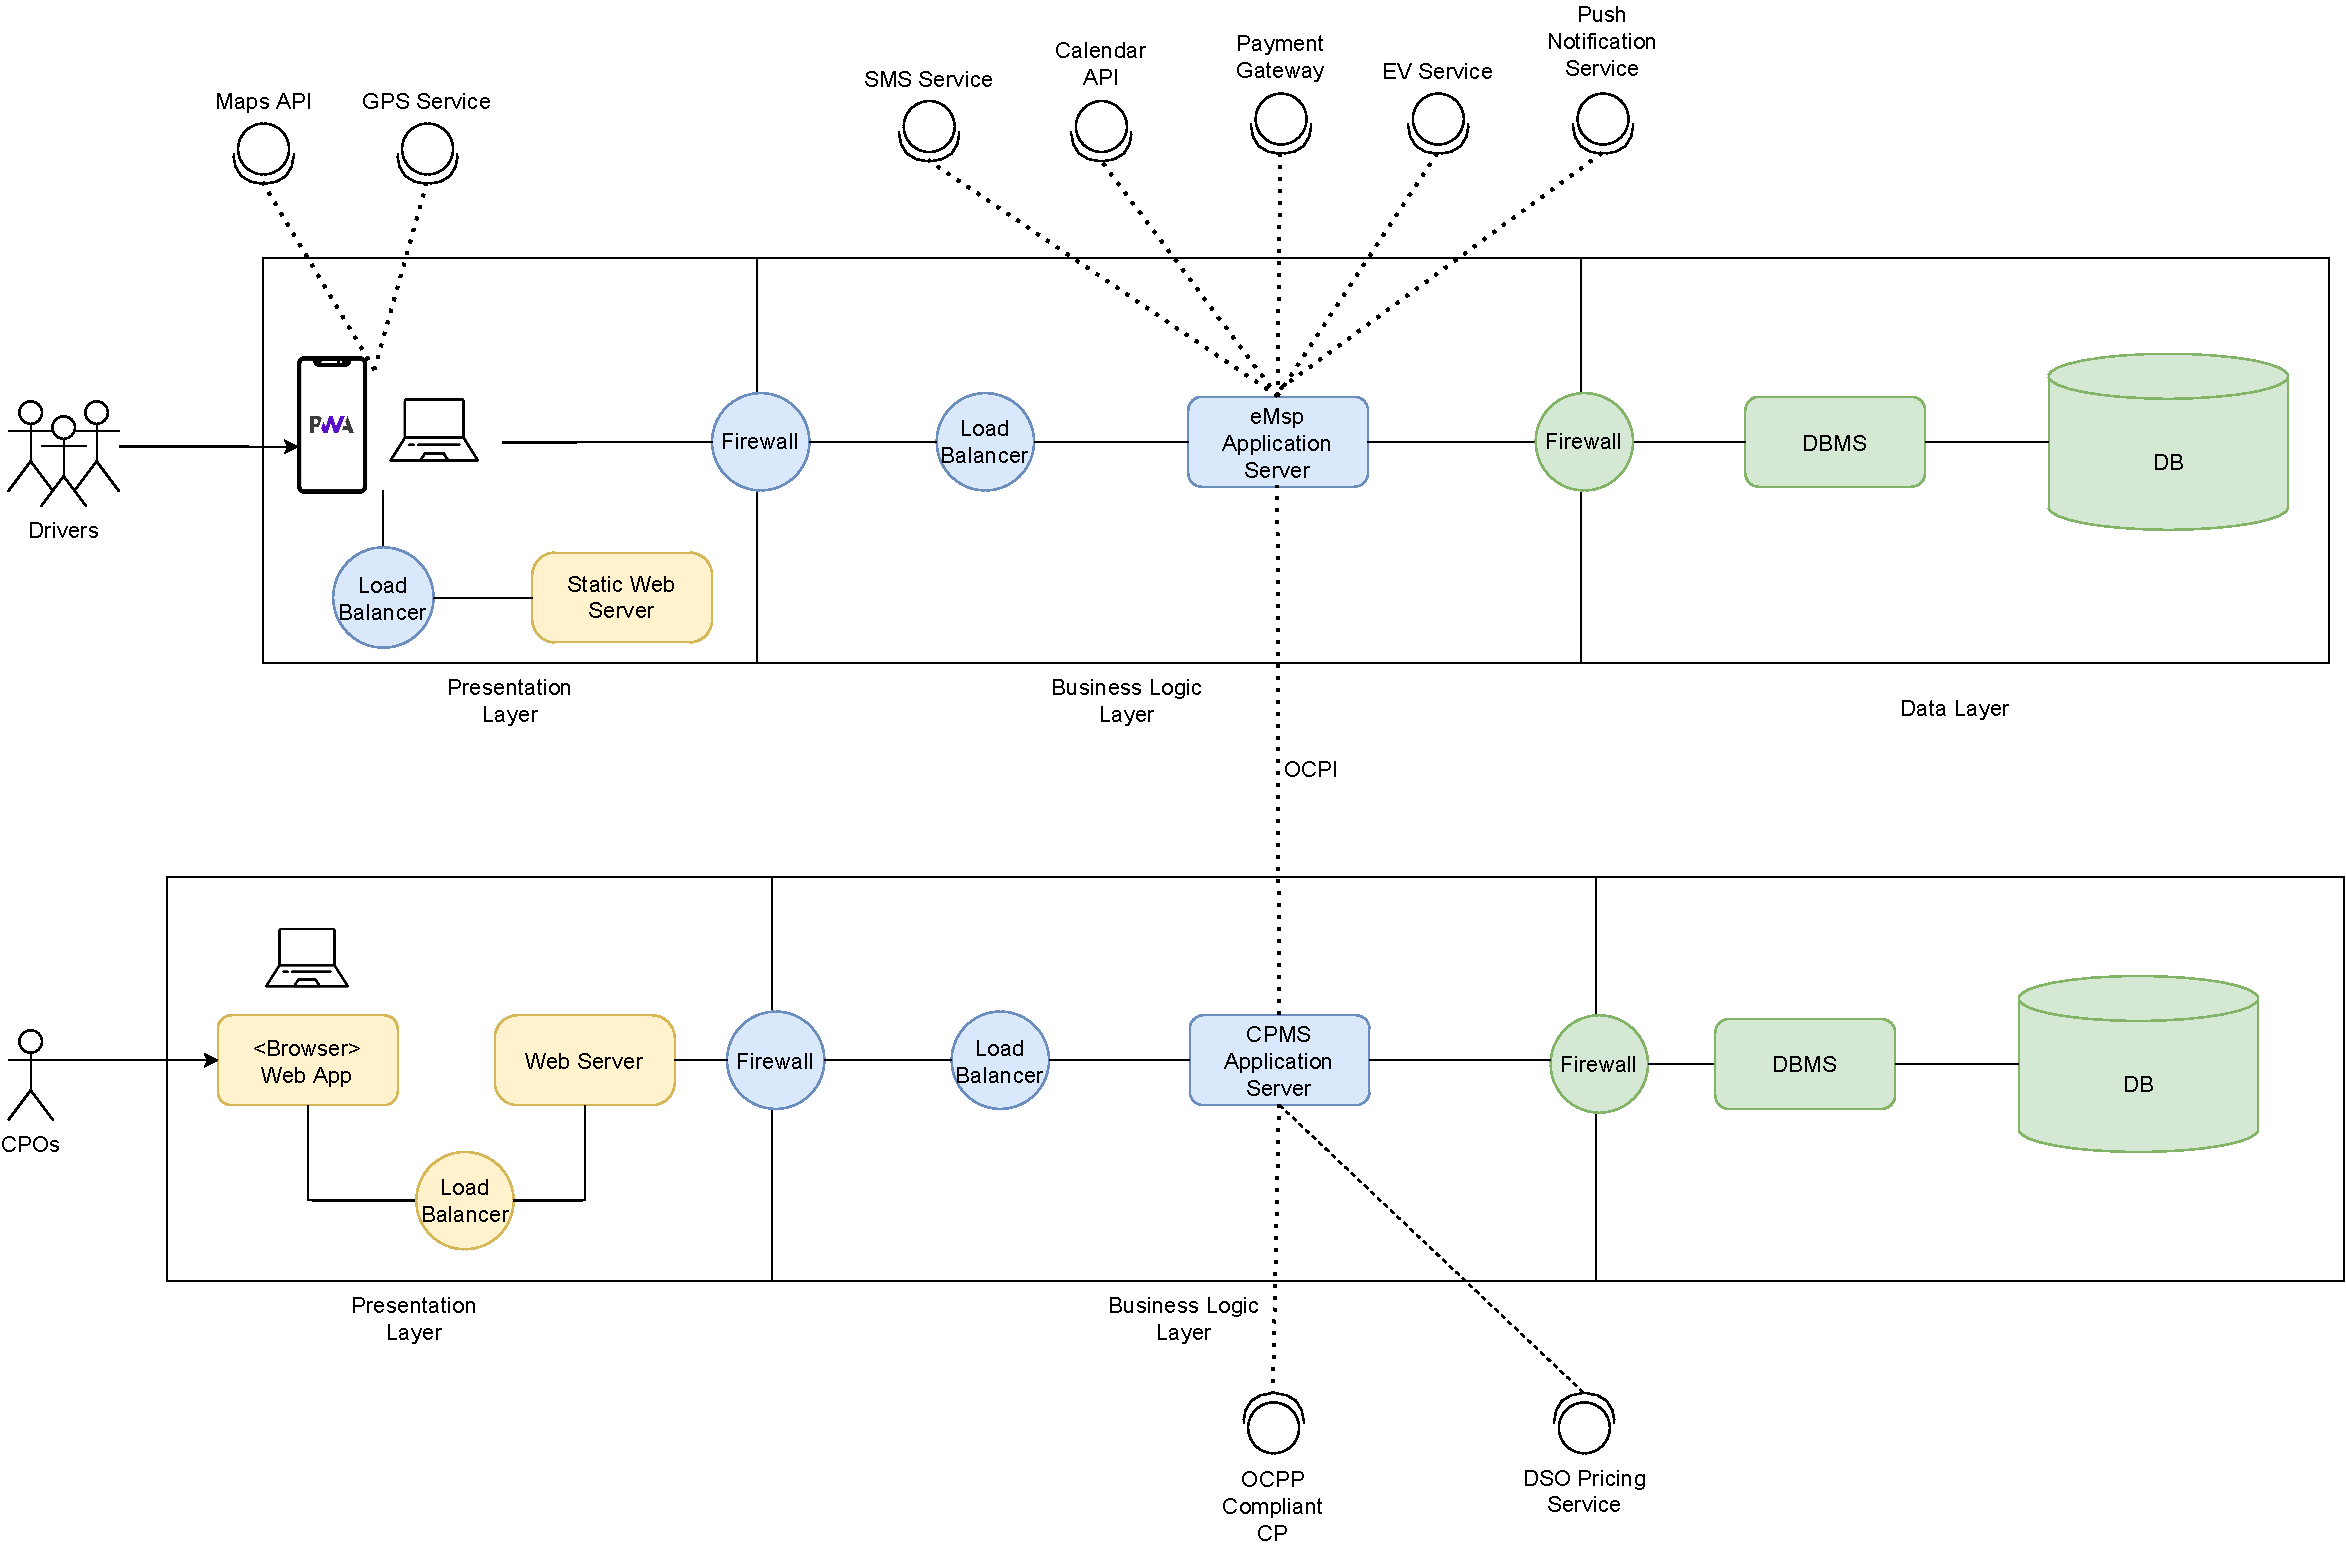
\includegraphics[scale=0.42]{src/Overview/overview_diagram.pdf}
\end{figure}

\hfill \\
The service is supposed to be accessed through a web interface.
Since the features offered and the intensity of the interaction with the application server
are very different depending on the type of user, the web interfaces will be developed following
different principles.
For the EV Drivers an SPA will be developed. An SPA is well-suited for applications
that require a lot of interaction and do not need to perform frequent full page reloads.
They can provide a faster and more seamless user experience for applications that require a
lot of interaction.
For the CPO an SSR Dashboard will be developed. SSR can provide a faster user experience
the server pre-renders the content, reducing the amount of work that the client needs to do.
The Overview Architecture of the S2B divides the application in the layers described
above, and contains some replicated Web Servers, which act as a middleware
between the user's browser and the application servers.
Finally, the application servers interfaces with the DBMS APIs, in order
to retrieve and store the data required for the considered computation.
The applications servers are expected to be stateless, according to the
REST standard definitions. The nodes are separated by firewalls to guarantee a higher level of security
of the whole system.

\begin{itemize}
    \item Static Web Server: it does not execute any business logic, but simply receive requests from the client and serve an HTML file along with other static assets (CSS Sheets, JS files, \dots).
          It does not route the request to the Application Server
    \item Web Server: it does not execute any business logic, but simply receive requests from the client, route
          them to the application servers which build the HTML page (along with the static assets) and send it back to the web server which serve the client
\end{itemize}
\pagebreak
\subsection{Component view}
In this section we show the components of the S2B, their relationships and interfaces. The following sections will explain the interaction between interfaces and details on each method of interfaces with REST endpoints, if any.

\begin{figure}[H]
    \centering
    \hspace*{-2cm}
    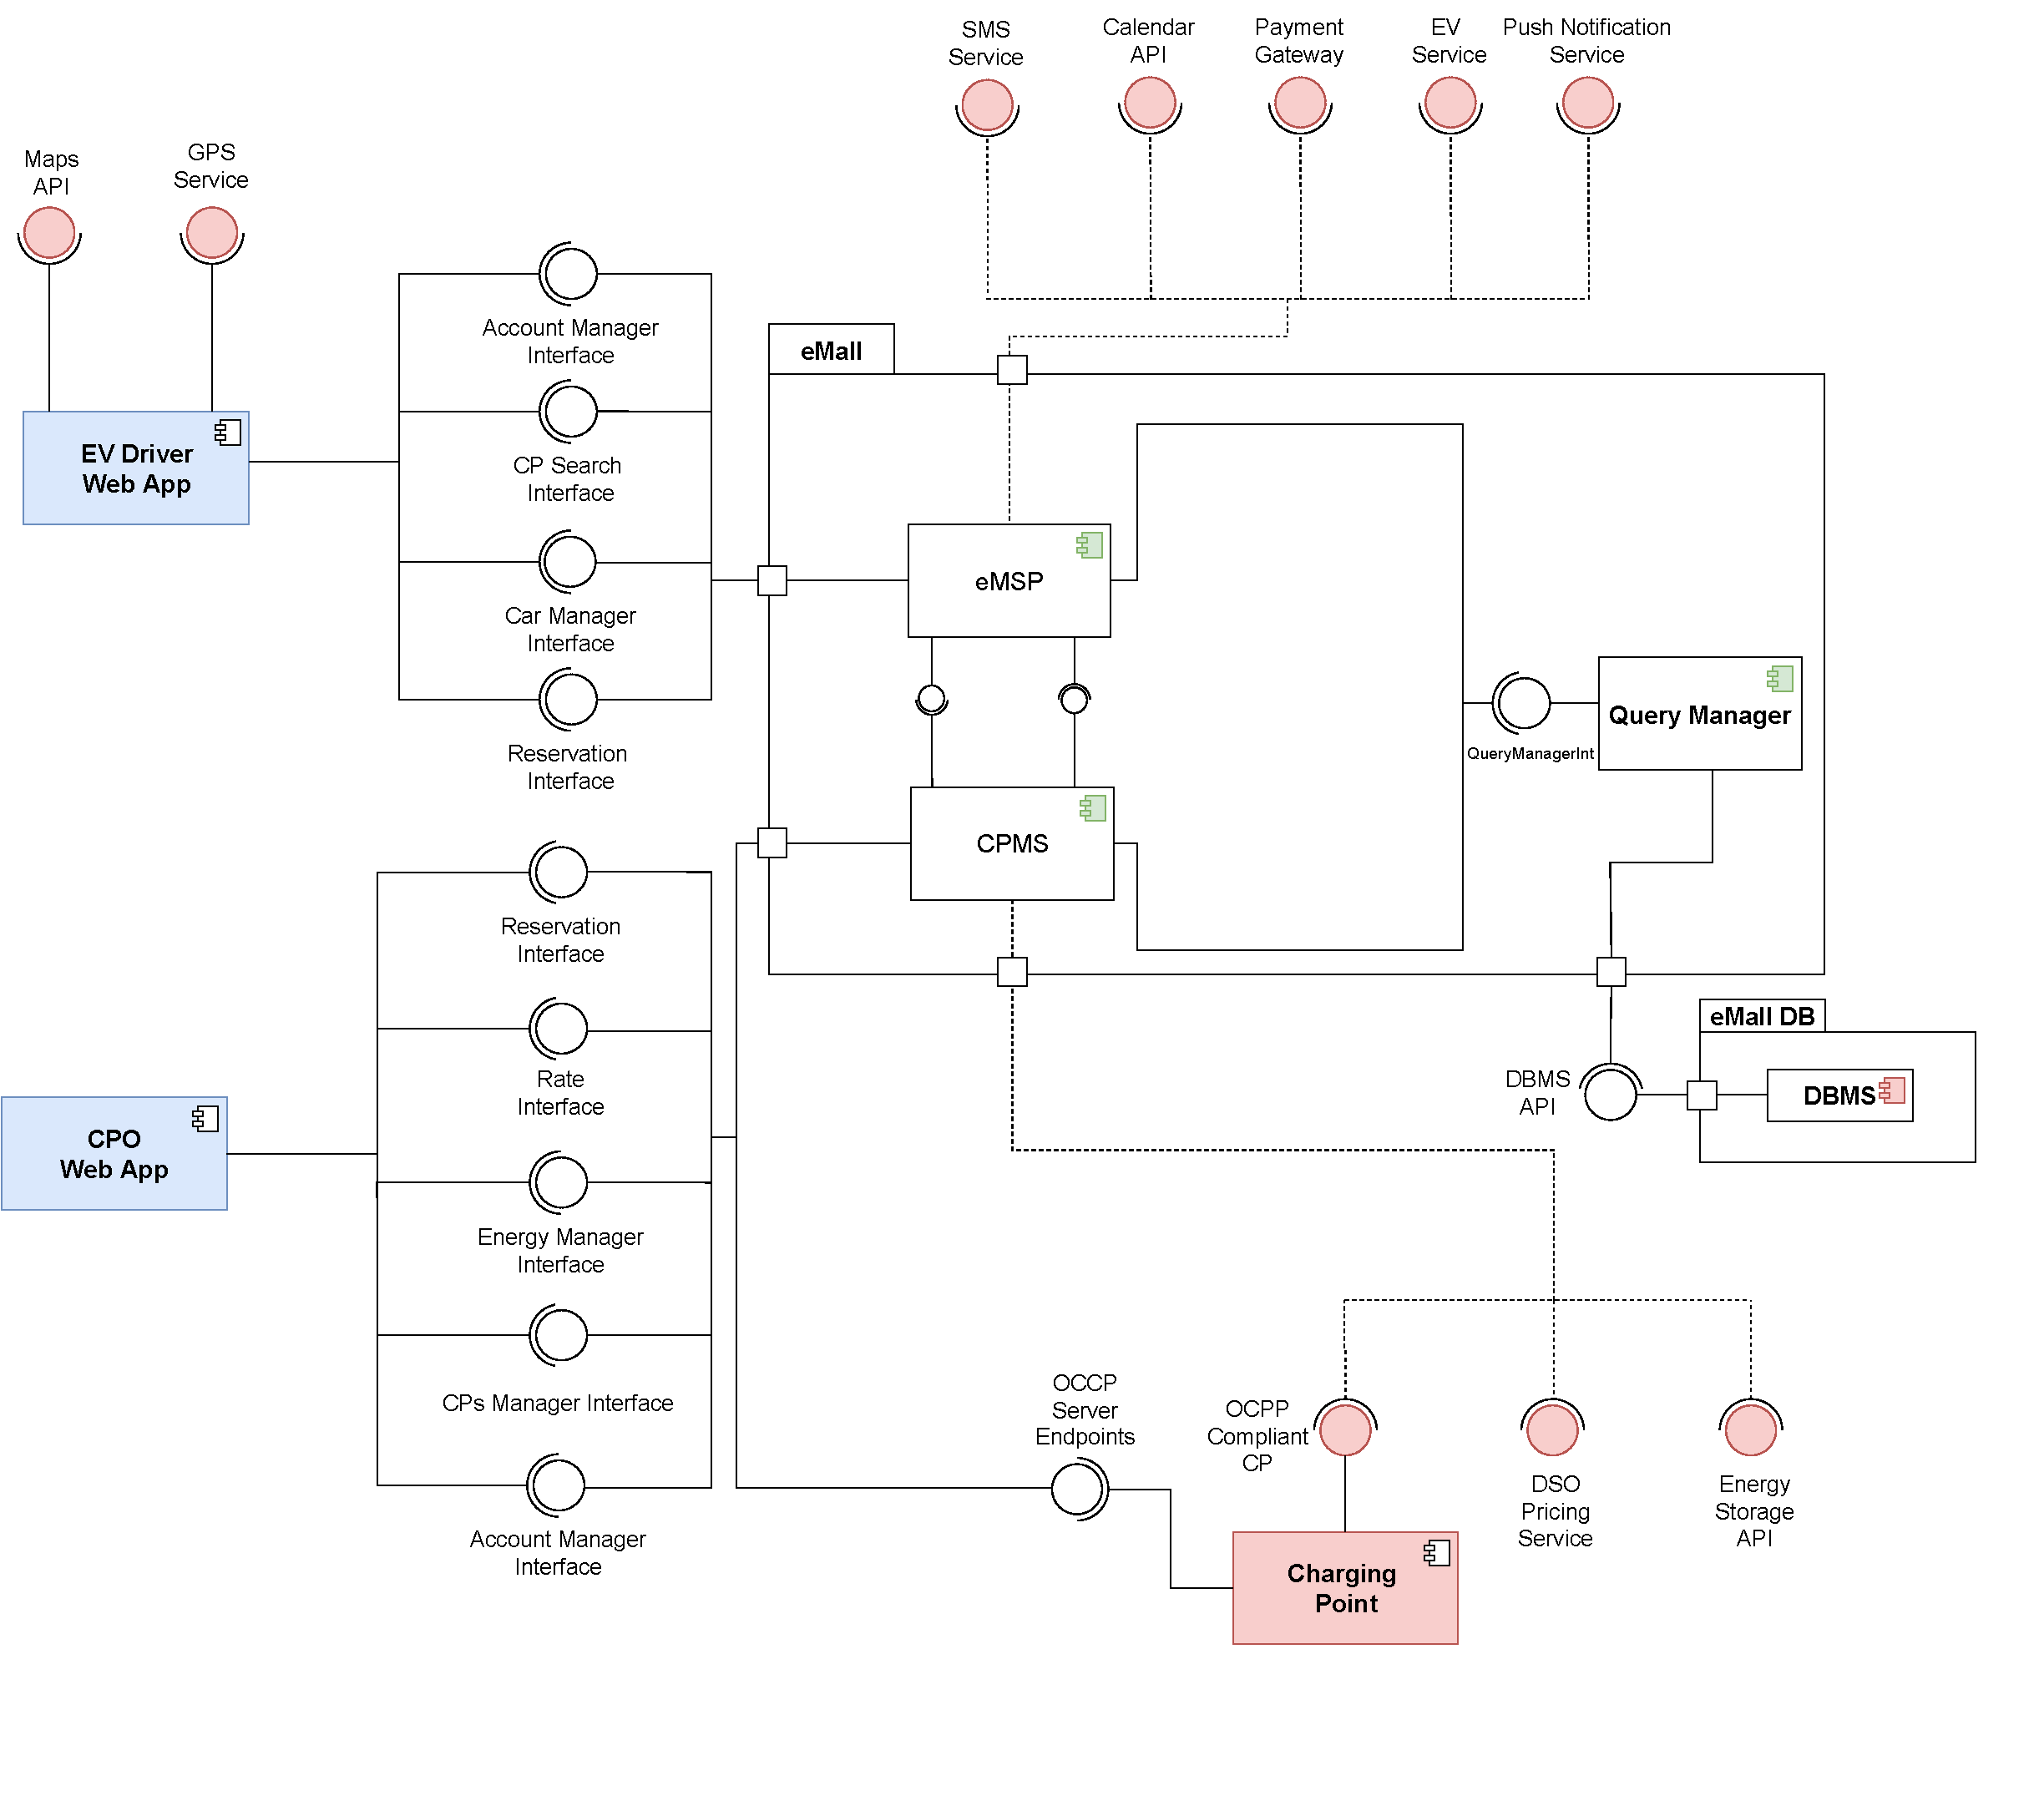
\includegraphics[scale=0.5]{src/ComponentDiagram/overview_component_diagram.pdf}
    \caption{Component Diagram of the eMall System}
\end{figure}


\subsubsection{eMSP}

\begin{figure}[H]
    \centering
    \hspace*{-2cm}
    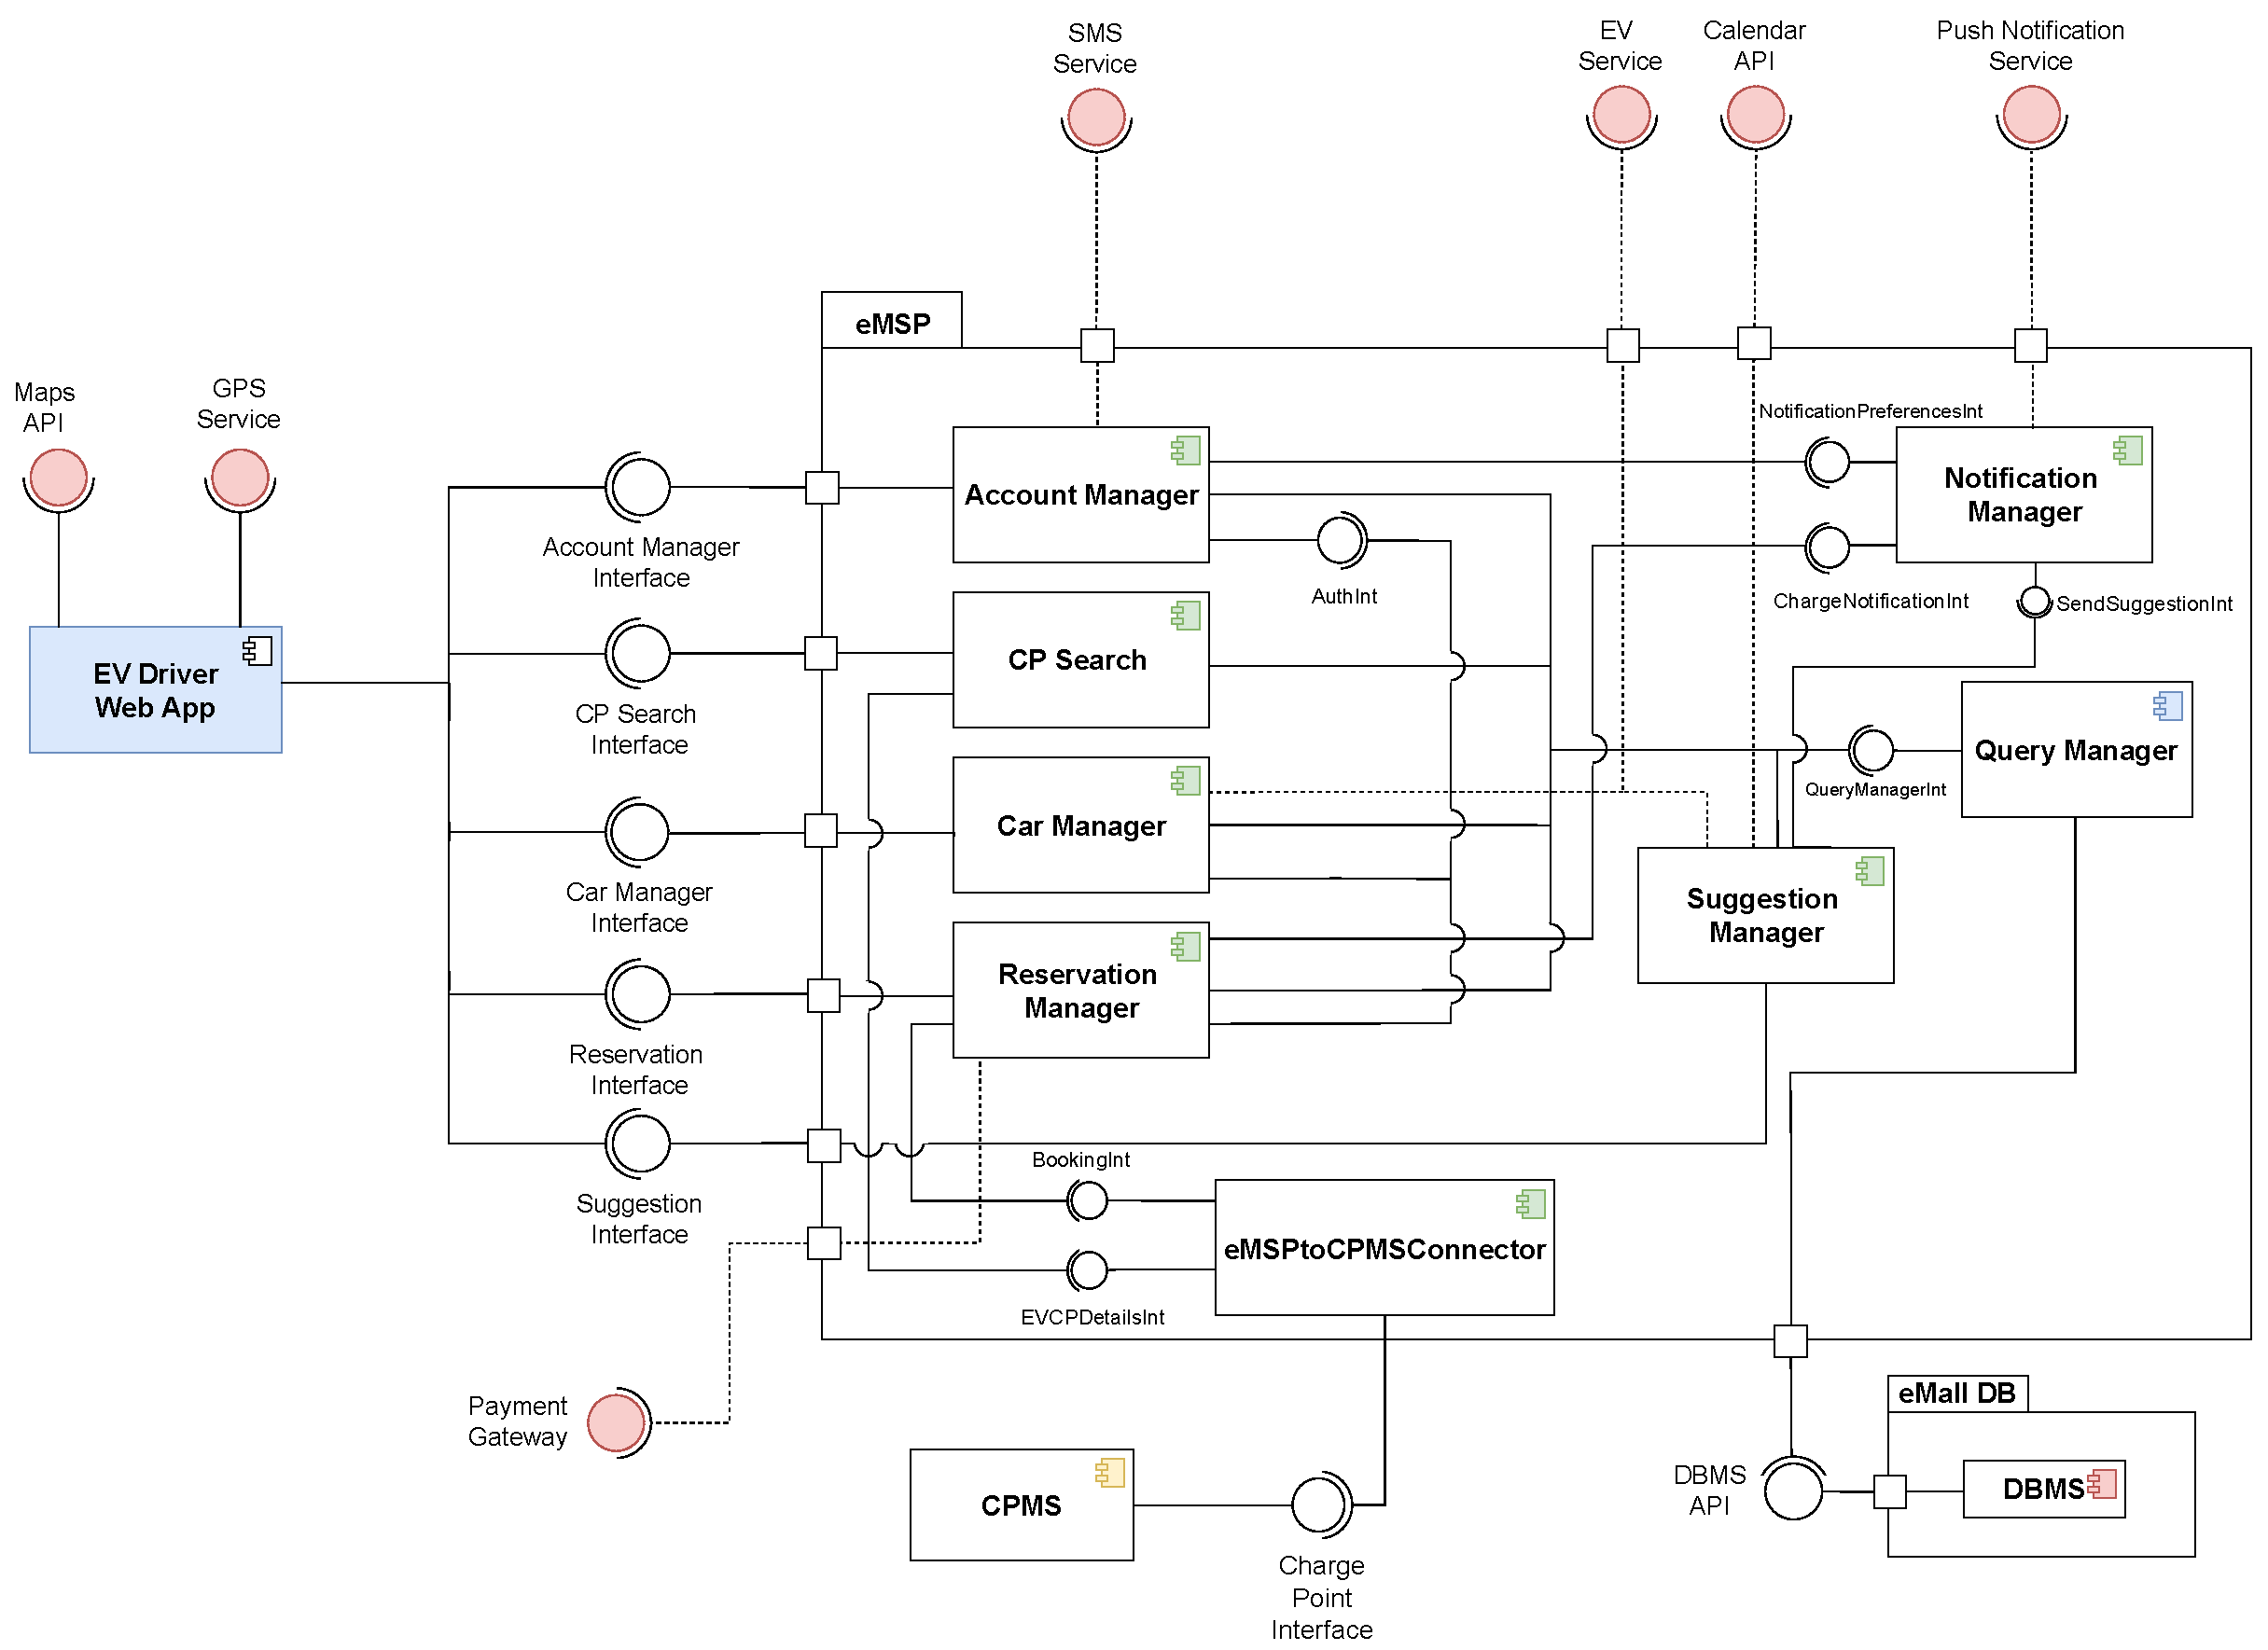
\includegraphics[scale=0.5]{src/ComponentDiagram/emsp_component_diagram.pdf}
    \caption{Component Diagram of the eMSP subsystem}
\end{figure}

\paragraph*{eMSP Web App} \hfill \\
It represents the application dedicated to the EV drivers. This component uses client side rendering of web pages. 
The user through the browser sends a request to the server and the eMSP Application Server responds with the HTML and Javascript which the browser then
downloads and execute. As the user interacts with the page, the Javascript can make additional requests to the server and update
the page dynamically, without need to fully reload the page. 
\paragraph*{eMSP Application Server} \hfill \\
The eMSP Application Server is responsible for the business logic to provide the functionality to the application for the EV Drivers and to coordinate the information flow between application layer and data layer
It is composed of several components, each of them used for a specific functionality:\\
\begin{itemize}
    \item \textbf{Account Manager} \\ This component handles all the account operations related to the CPO and offers an interface to authenticate
          the requests in the CPMS application server.
          It offers functionality to create new account, logging in, setting preferences and verify the authentication of the user at any time.
          To create a new account interacts with the external SMS API to make the user receive a code to verify the identity.
    \item \textbf{CP Search} \\ This component handles the operations needed to show the CPs in a specified range of km near a location. The location
        can be described as an address, with coordinates or by geolocating the actual position of the incoming request. It selects the filtered CPs that are then 
        shown in the map as placeholders.  
    \item \textbf{Car Manager} \\ This component handles the operations related to the status of the car. It offers an interface to select the EV model among a list of 
        all the marketed models and offers an interface to connect the car to the application. It uses these information to show the battery status of the EV, the 
        amount of power during a charging process and to suggest charging plans based on the specific vehicle and status of it.
    \item \textbf{Reservation Manager} \\ This component handles all the operations related to the reservations for the EV Drivers. It offers the possibility to create a reservation
    for a charge and pay for that reservation, see the details of a reservation, start or pause a charge of a particular reservation and see the recap of an already occurred reservation.
    It permits to pay for a reservation using an external Payment Gateway that handles all the payment process and returns the status of the payment.  

\end{itemize}


\subsubsection{CPMS}

\begin{figure}[H]
    \centering
    \hspace*{-2cm}
    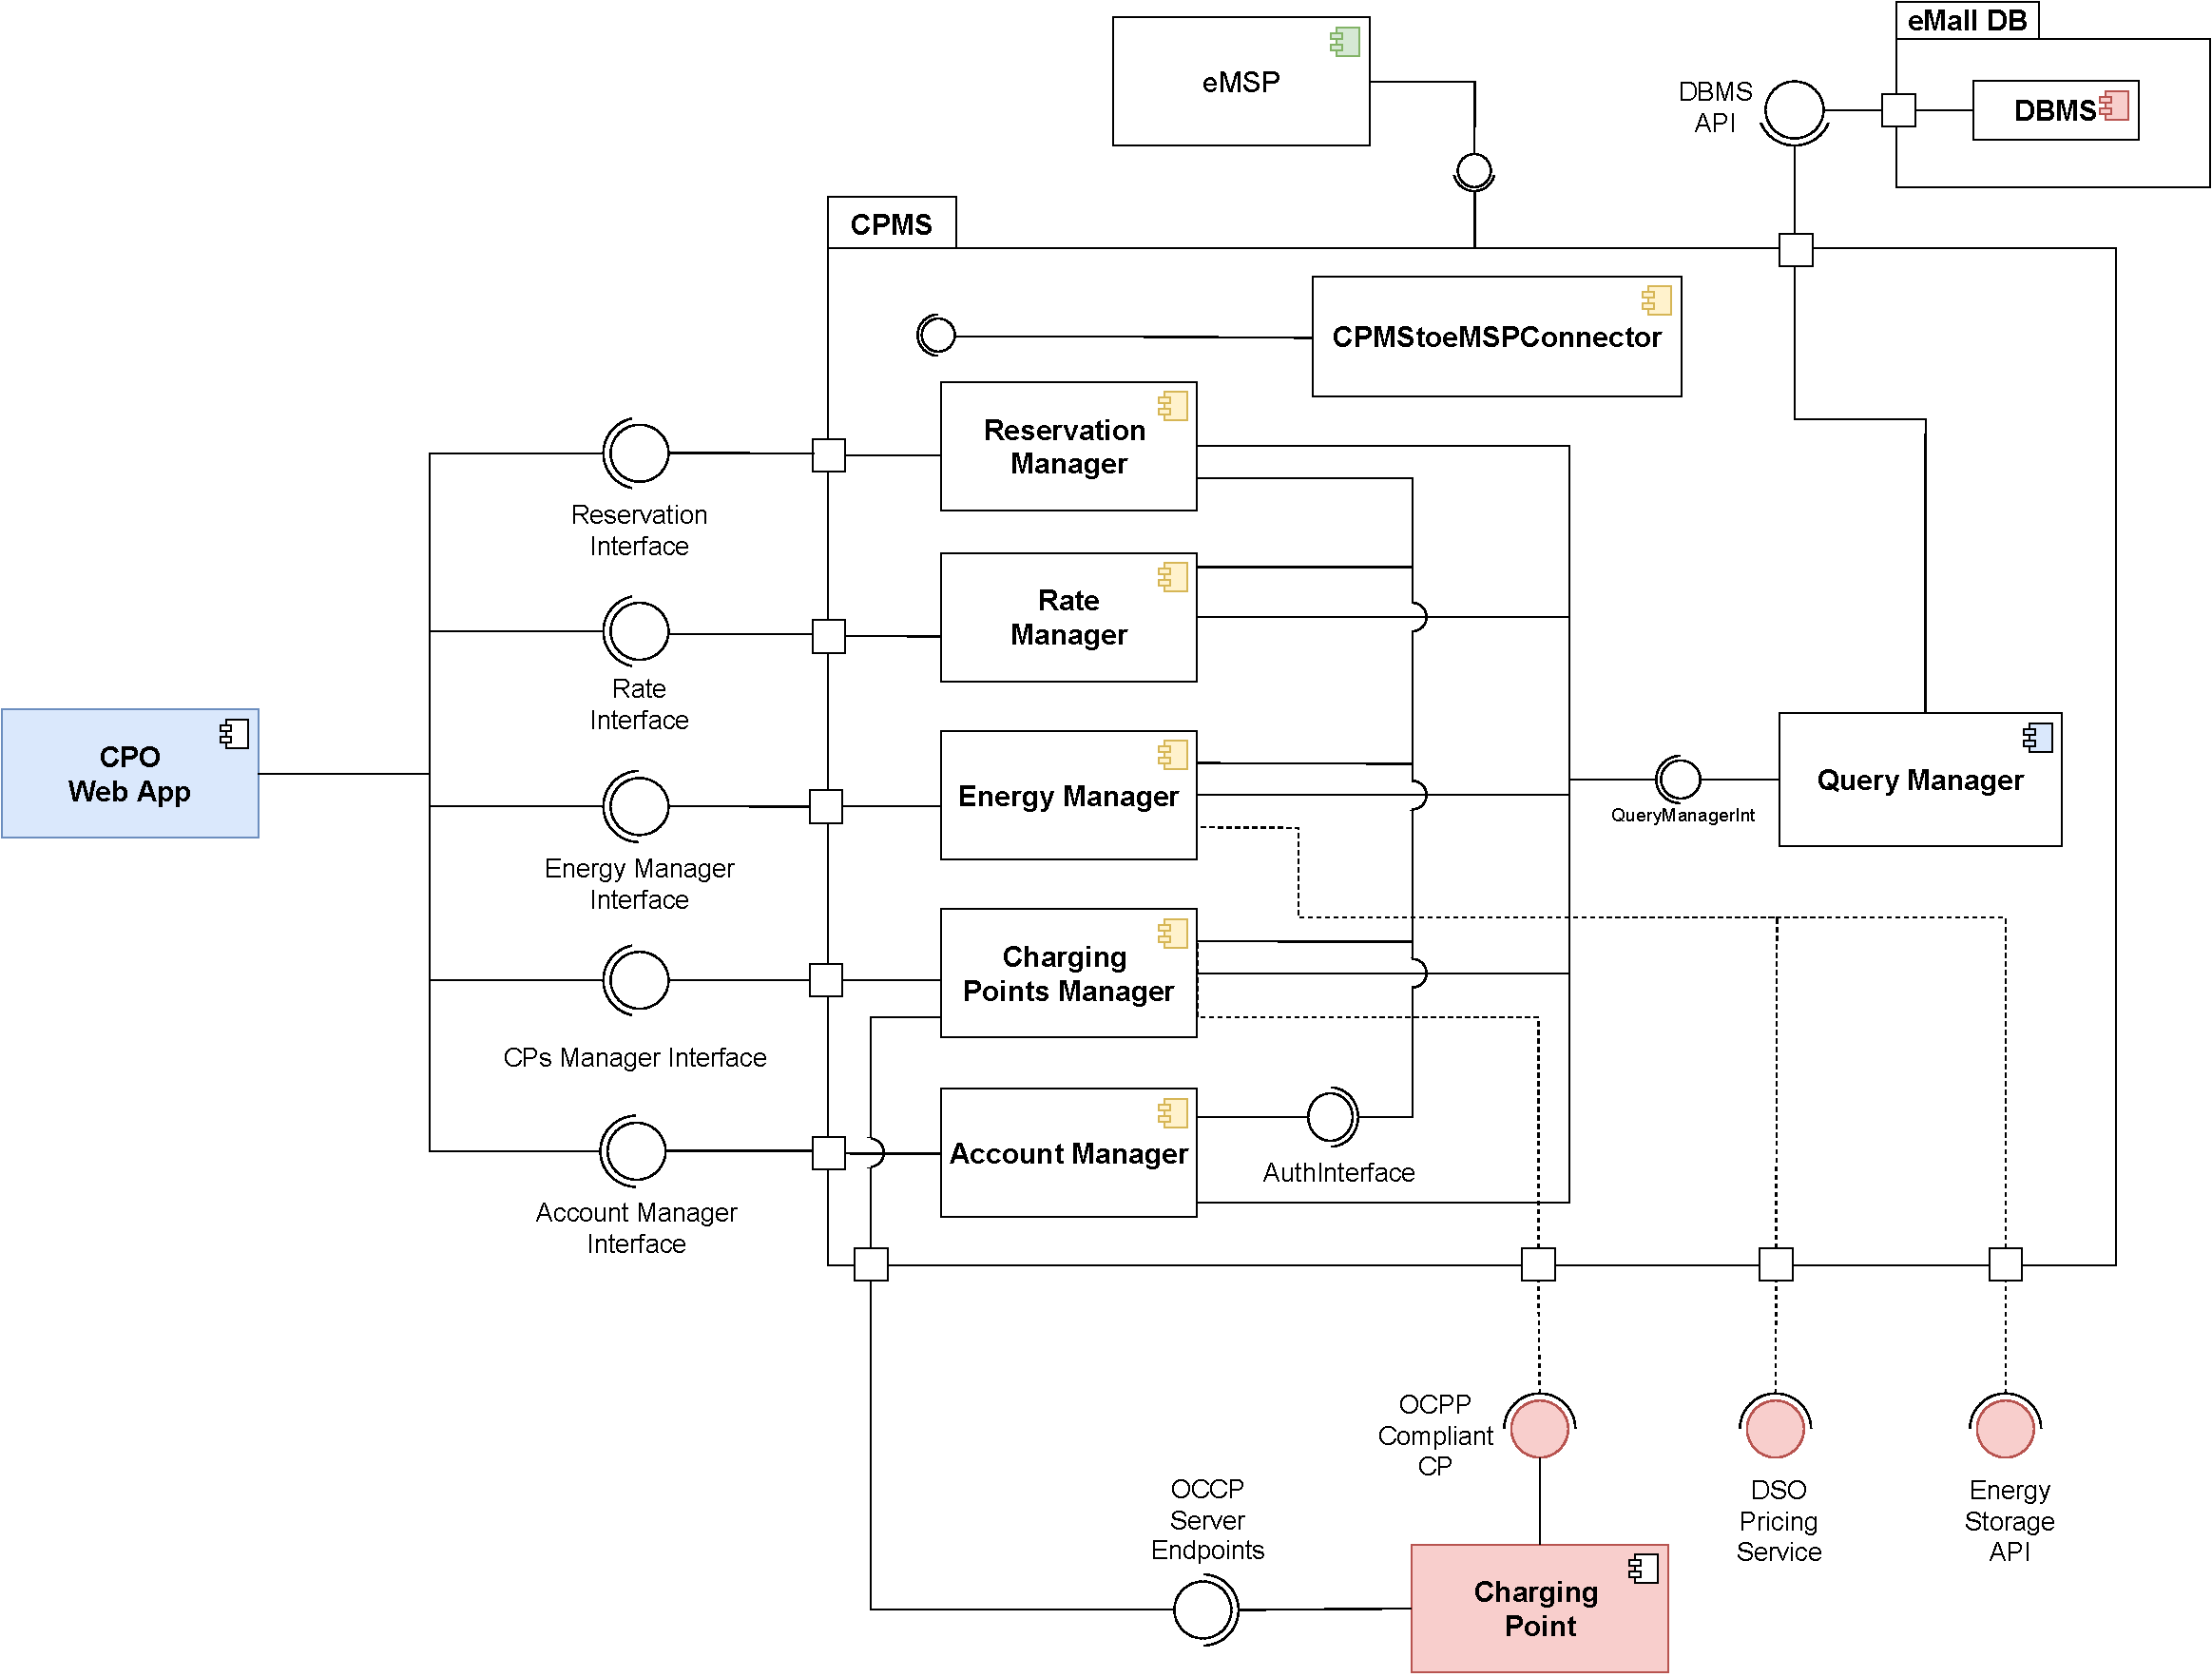
\includegraphics[scale=0.5]{src/ComponentDiagram/cpms_component_diagram.pdf}
    \caption{Component Diagram of the CPMS subsystem}
\end{figure}

\paragraph*{CPO Web App} \hfill \\
It represents the application dedicated to the different CPOs using the system. This component contains the logic to receive HTTPS requests from the users' browser,
forward them to the CPMS Application Server, and generate dynamic pages based on the response from the CPMS Application Server.

\paragraph*{CPMS Application Server} \hfill \\
The CPMS Application Server is responsible for the business logic to provide the functionality to the application for the CPOs and to coordinate the information flow between application layer and data layer.
It is composed of several components, each of them used for a specific functionality:\\
\begin{itemize}
    \item \textbf{Booking Manager} \\
    This component handles the operations regarding the reservation of a specific CPO. It offers the possibility to manage the reservations and to control their status.
    \item \textbf{Rate Manager} \\ This component is responsible for the operations regarding the rates of that are associated with the CPs. It offers the possibility to
    create a new rate in all its details, to add a special rate and specify the duration. The created rates then are associated to a specific CP.
    \item \textbf{Energy Manager} \\ This component is responsible for the operations regarding the managing of the energy of the different EVCPs. 
    It offers the possibility to verify the energy consumption and production of the different sources, modify and visualize the status of the energy storage system,
    visualize the availability of energy contracts provided by the DSOs for a specific EVCP and stipulate a contract among the ones available.
    \item \textbf{Charging Points Manager} \\ This component handles the operations regarding the managing of the CPs. It is an OCPP server for the CPs, offering the 
    required functionalities for adding and removing a CP, for starting and stopping a charge and for receiving status data by the CP. It offers an interface to connect the different CPs through their platform.
    \item \textbf{Account Manager} \\ This component handles all the account operations related to the CPO and offers an interface to authenticate the requests in the CPMS application server.
          It offers functionality to create new account, logging in, setting preferences and verify the authentication of the user at any time.
          To create a new account interacts with the external SMS API to make the user receive a code to verify the identity.
\end{itemize}

\begin{figure}[H]
    \centering
    \hspace*{-2.5cm}
    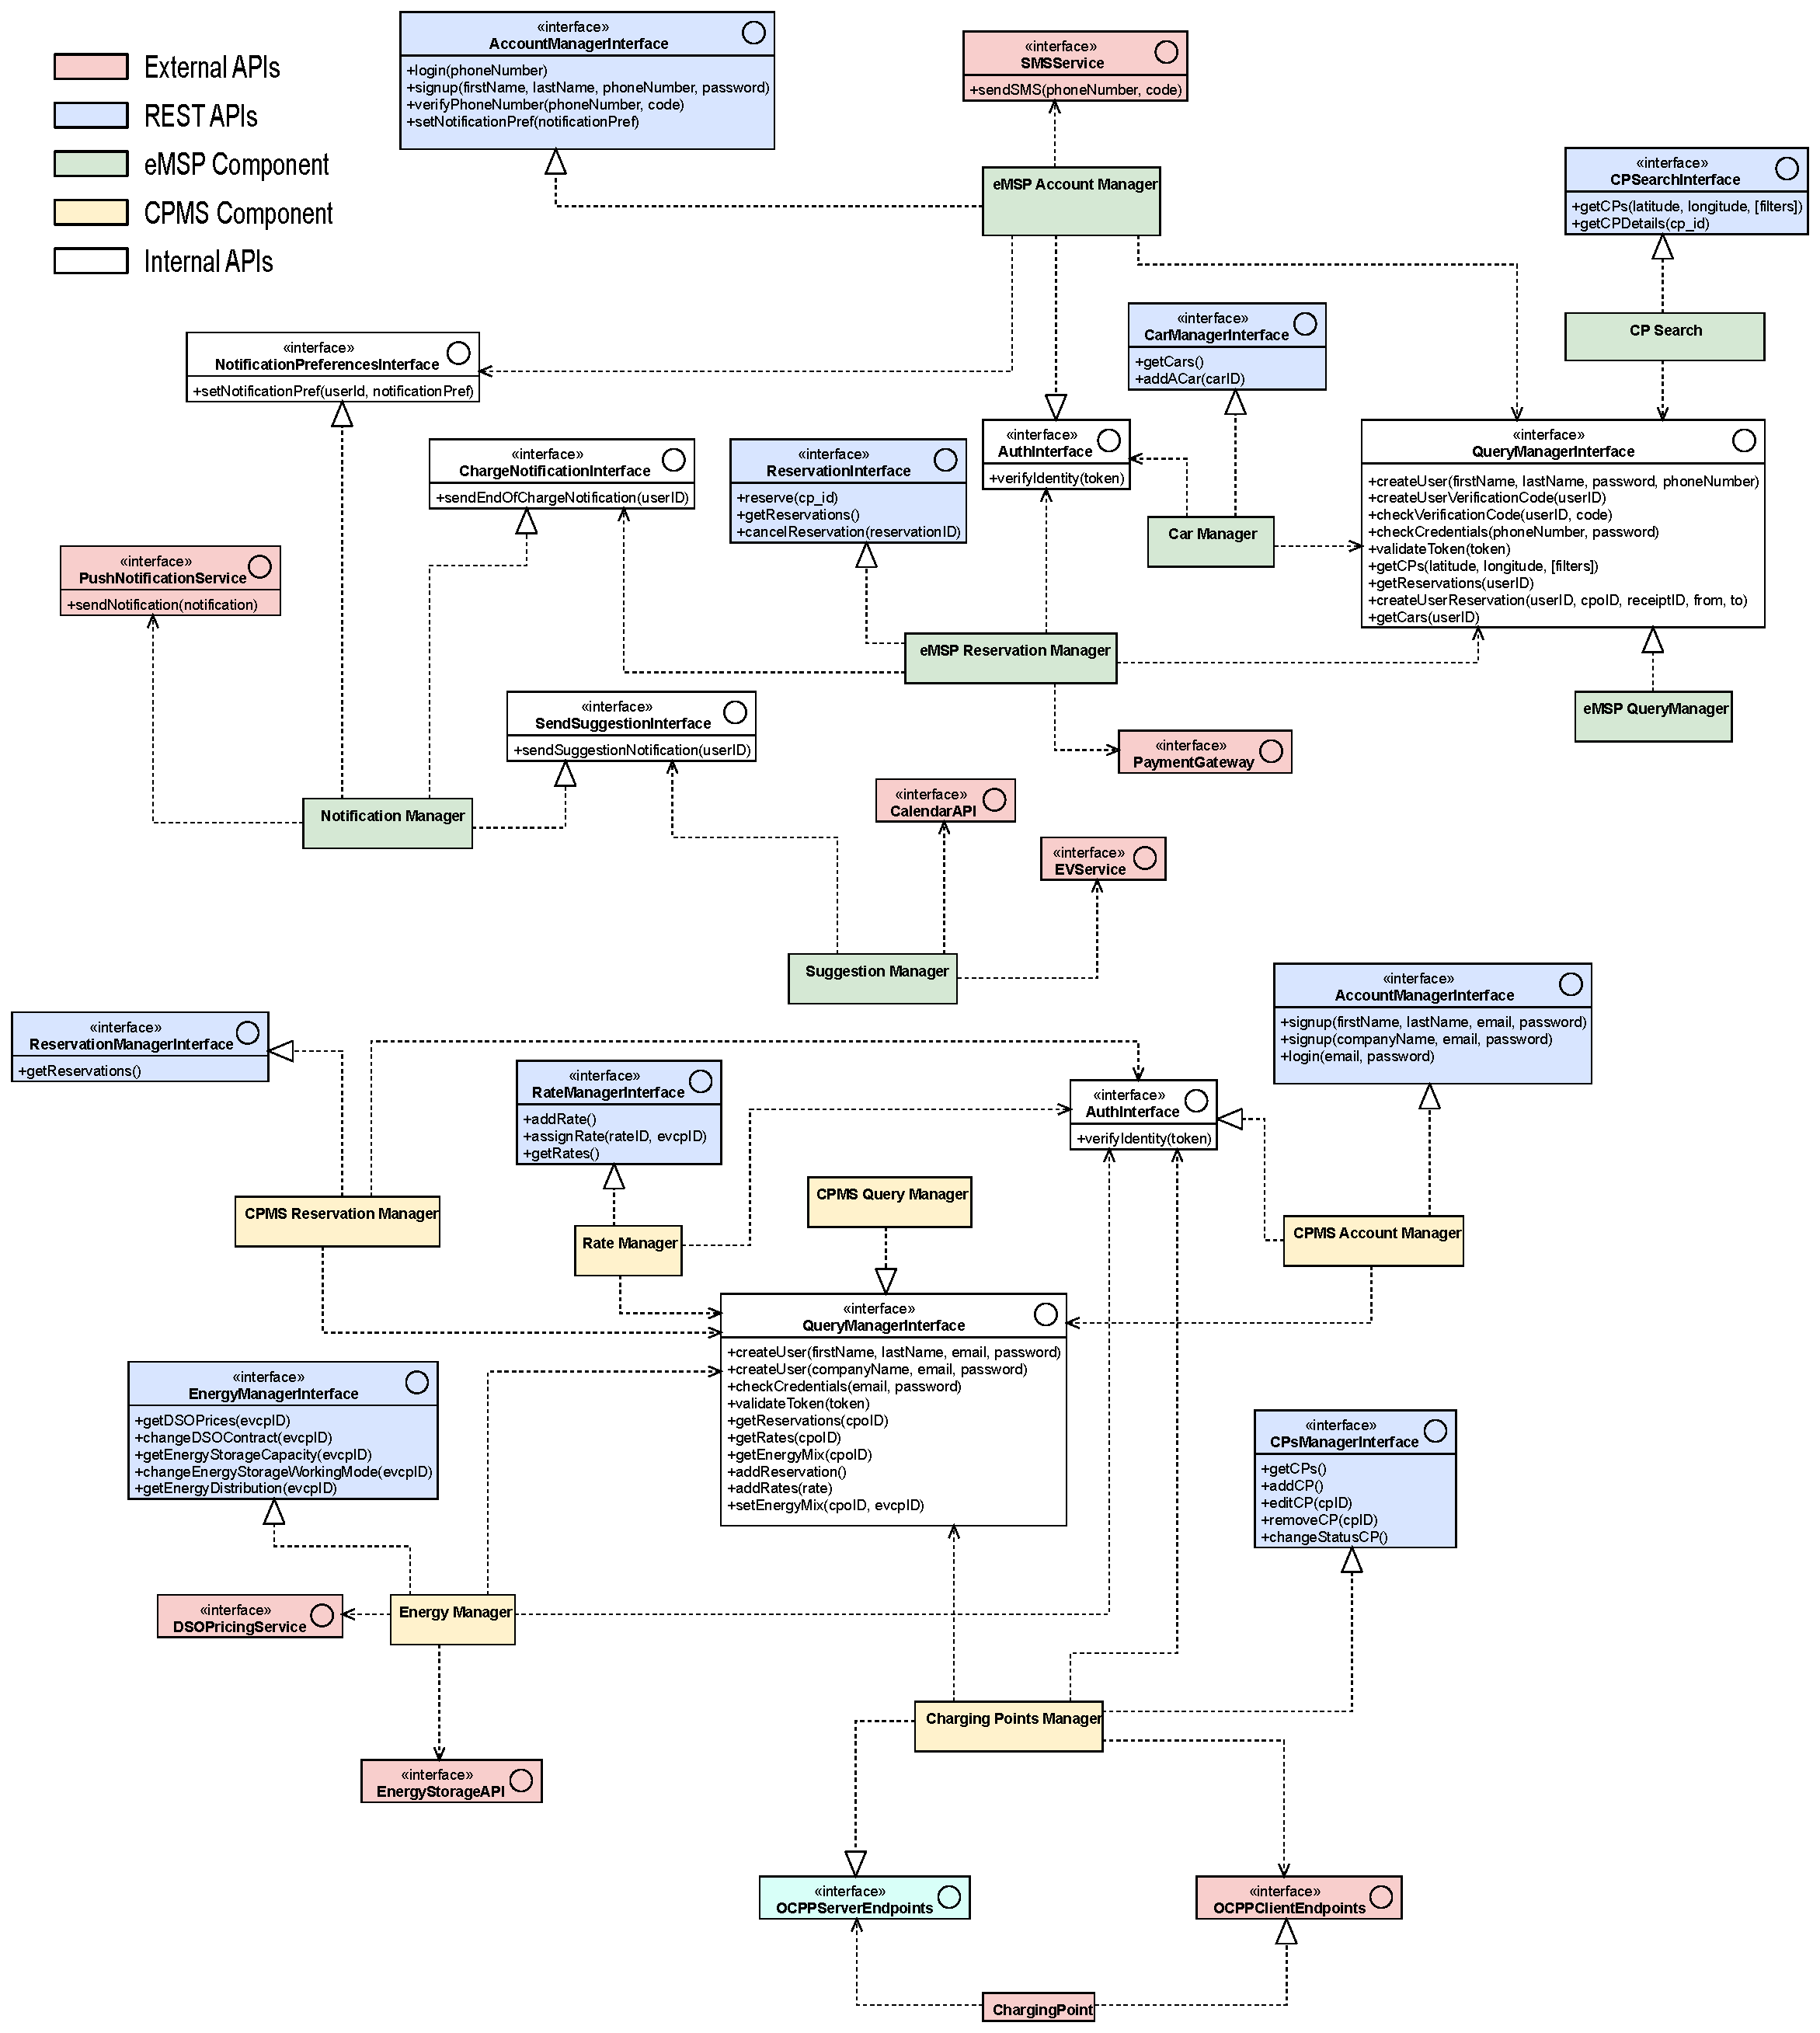
\includegraphics[height=\textheight-1.5cm,keepaspectratio]{src/componentInterfaces/component_interface.pdf}
    \caption{Class Diagram with interfaces of the eMall System}
\end{figure}


\subsubsection{Logical Description of Data}
\begin{figure}[H]
    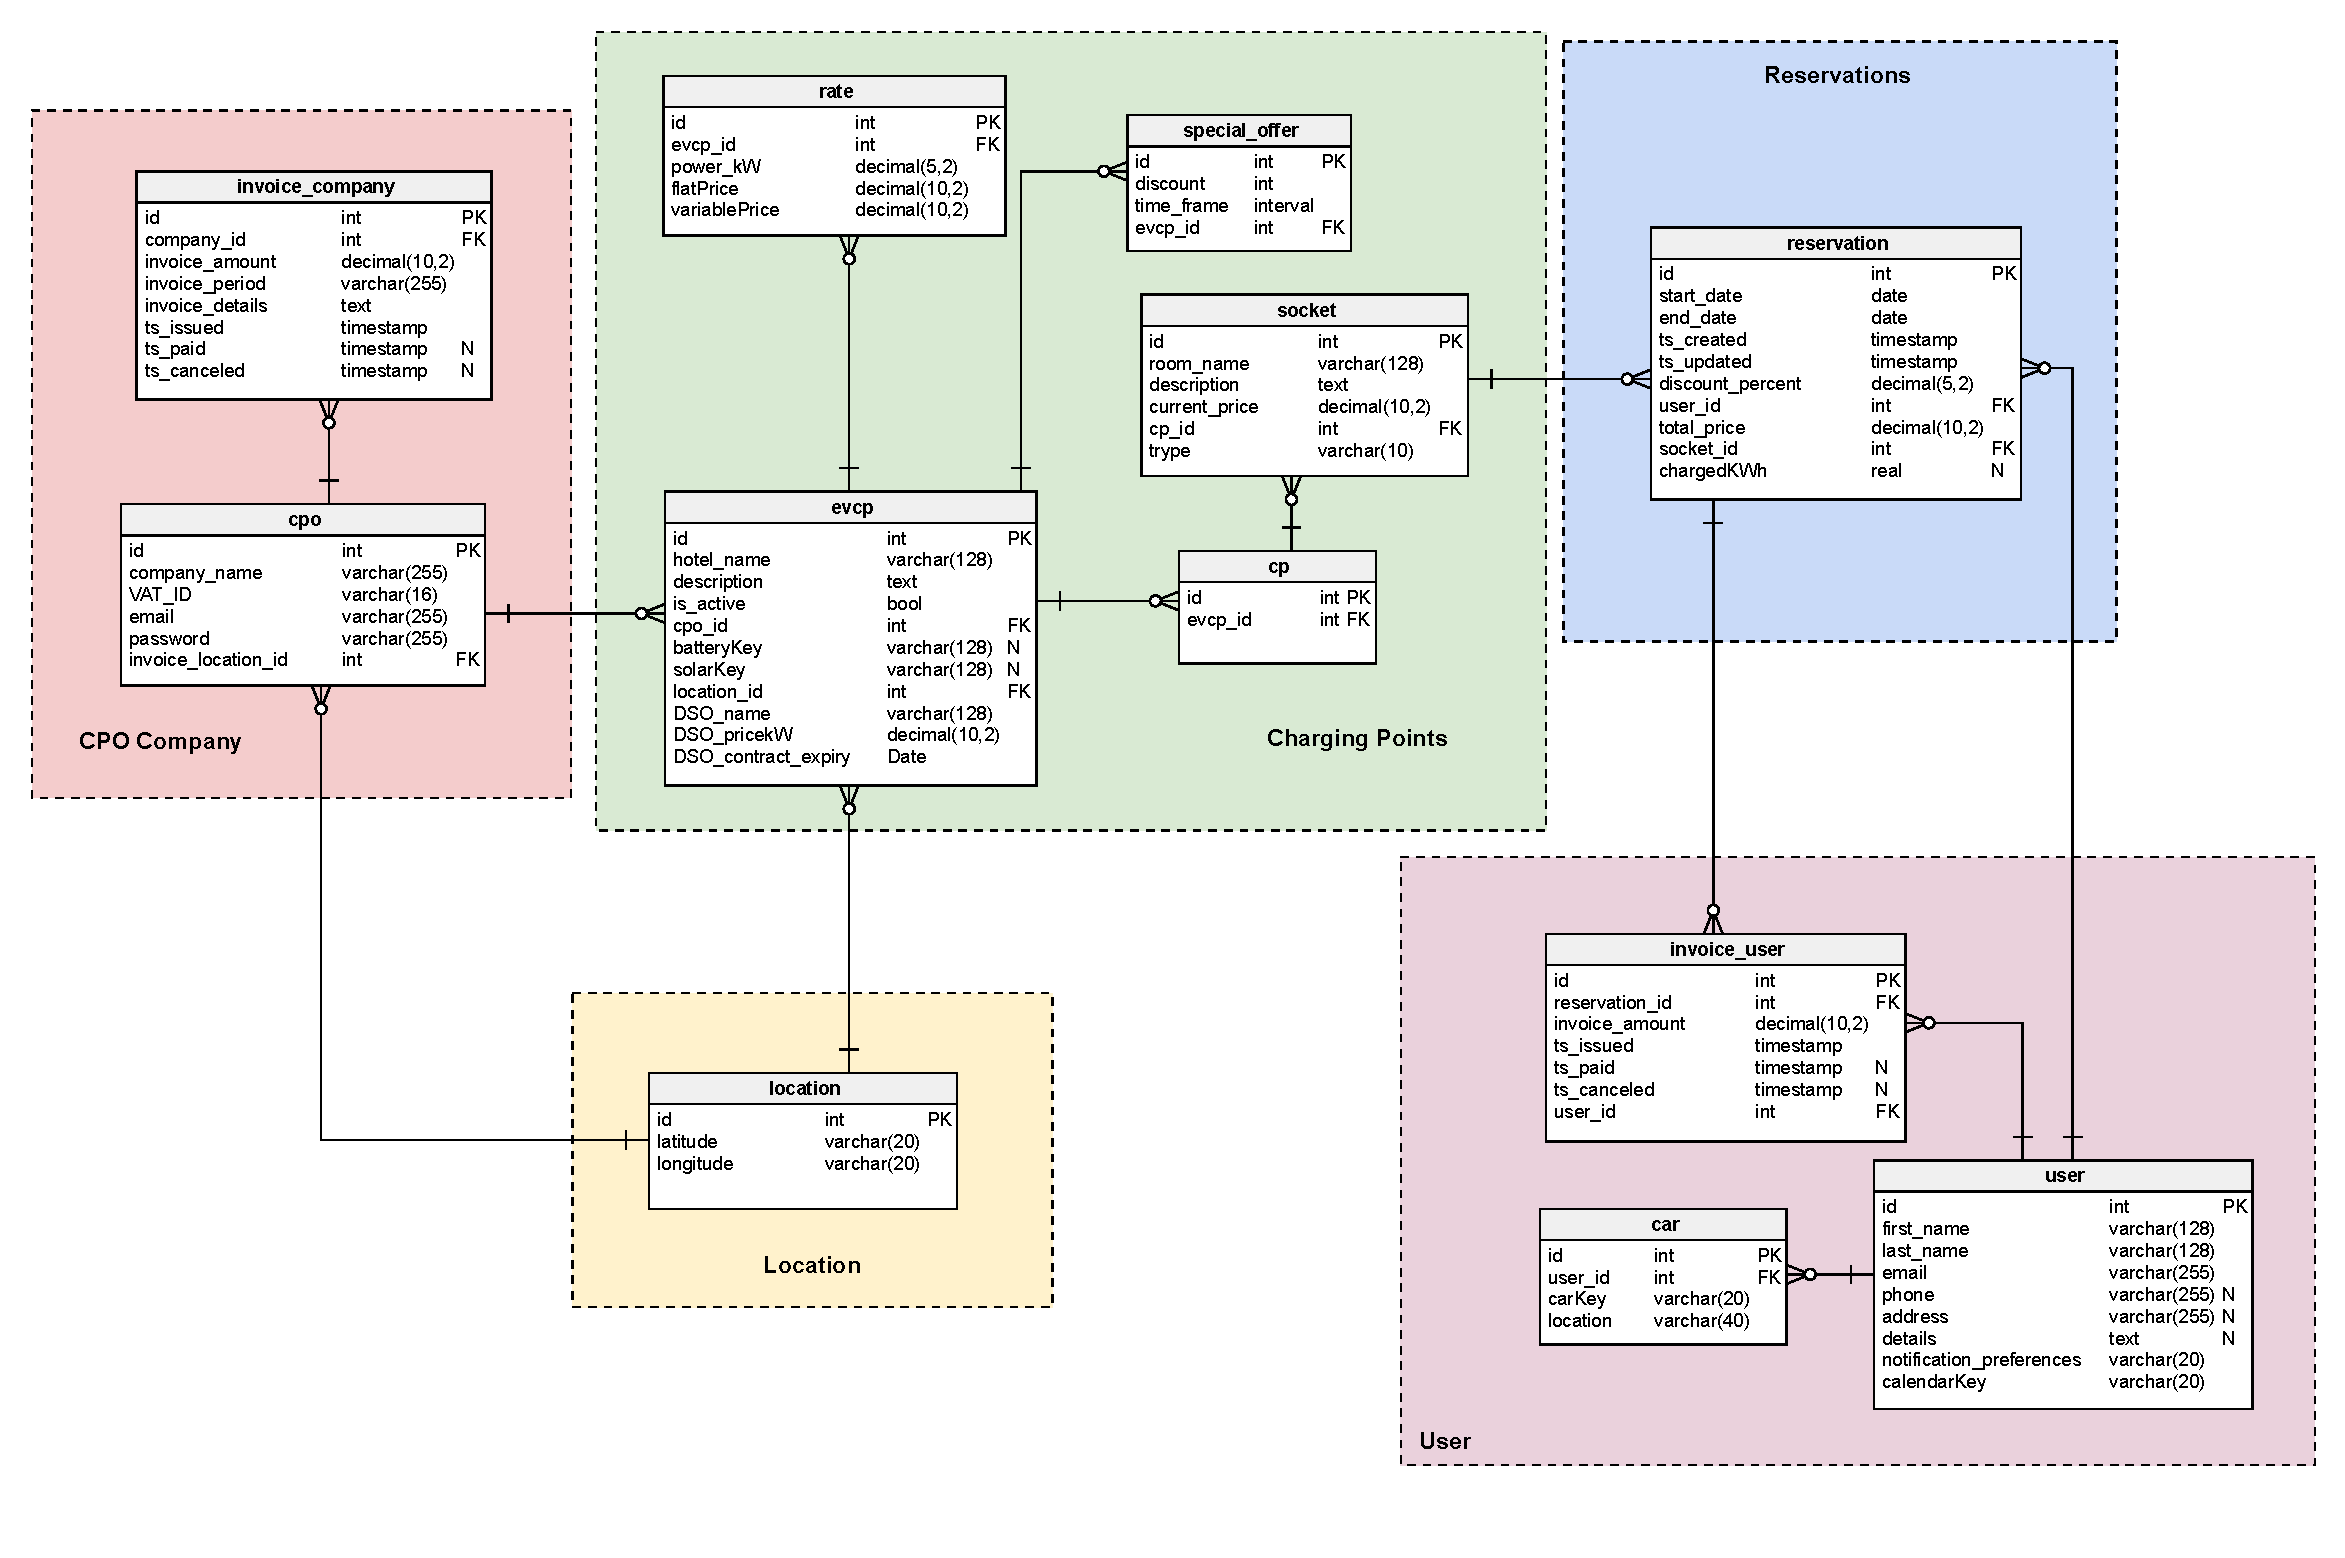
\includegraphics[scale=0.30]{src/ERDiagram/er_diagram.pdf}
\end{figure}

\subsection{Deployment view}
Infrastructure: deployment diagram(s) including non-logical elements (e.g., load balancer, firewall)

\subsection{Runtime view}
You can use sequence diagrams to describe the way components interact to accomplish specific tasks typically related to your use cases. Dynamics of the interactions: sequence
diagrams (realization of use cases)

\subsubsection{eMSP}
\begin{figure}[H]
    \centering
    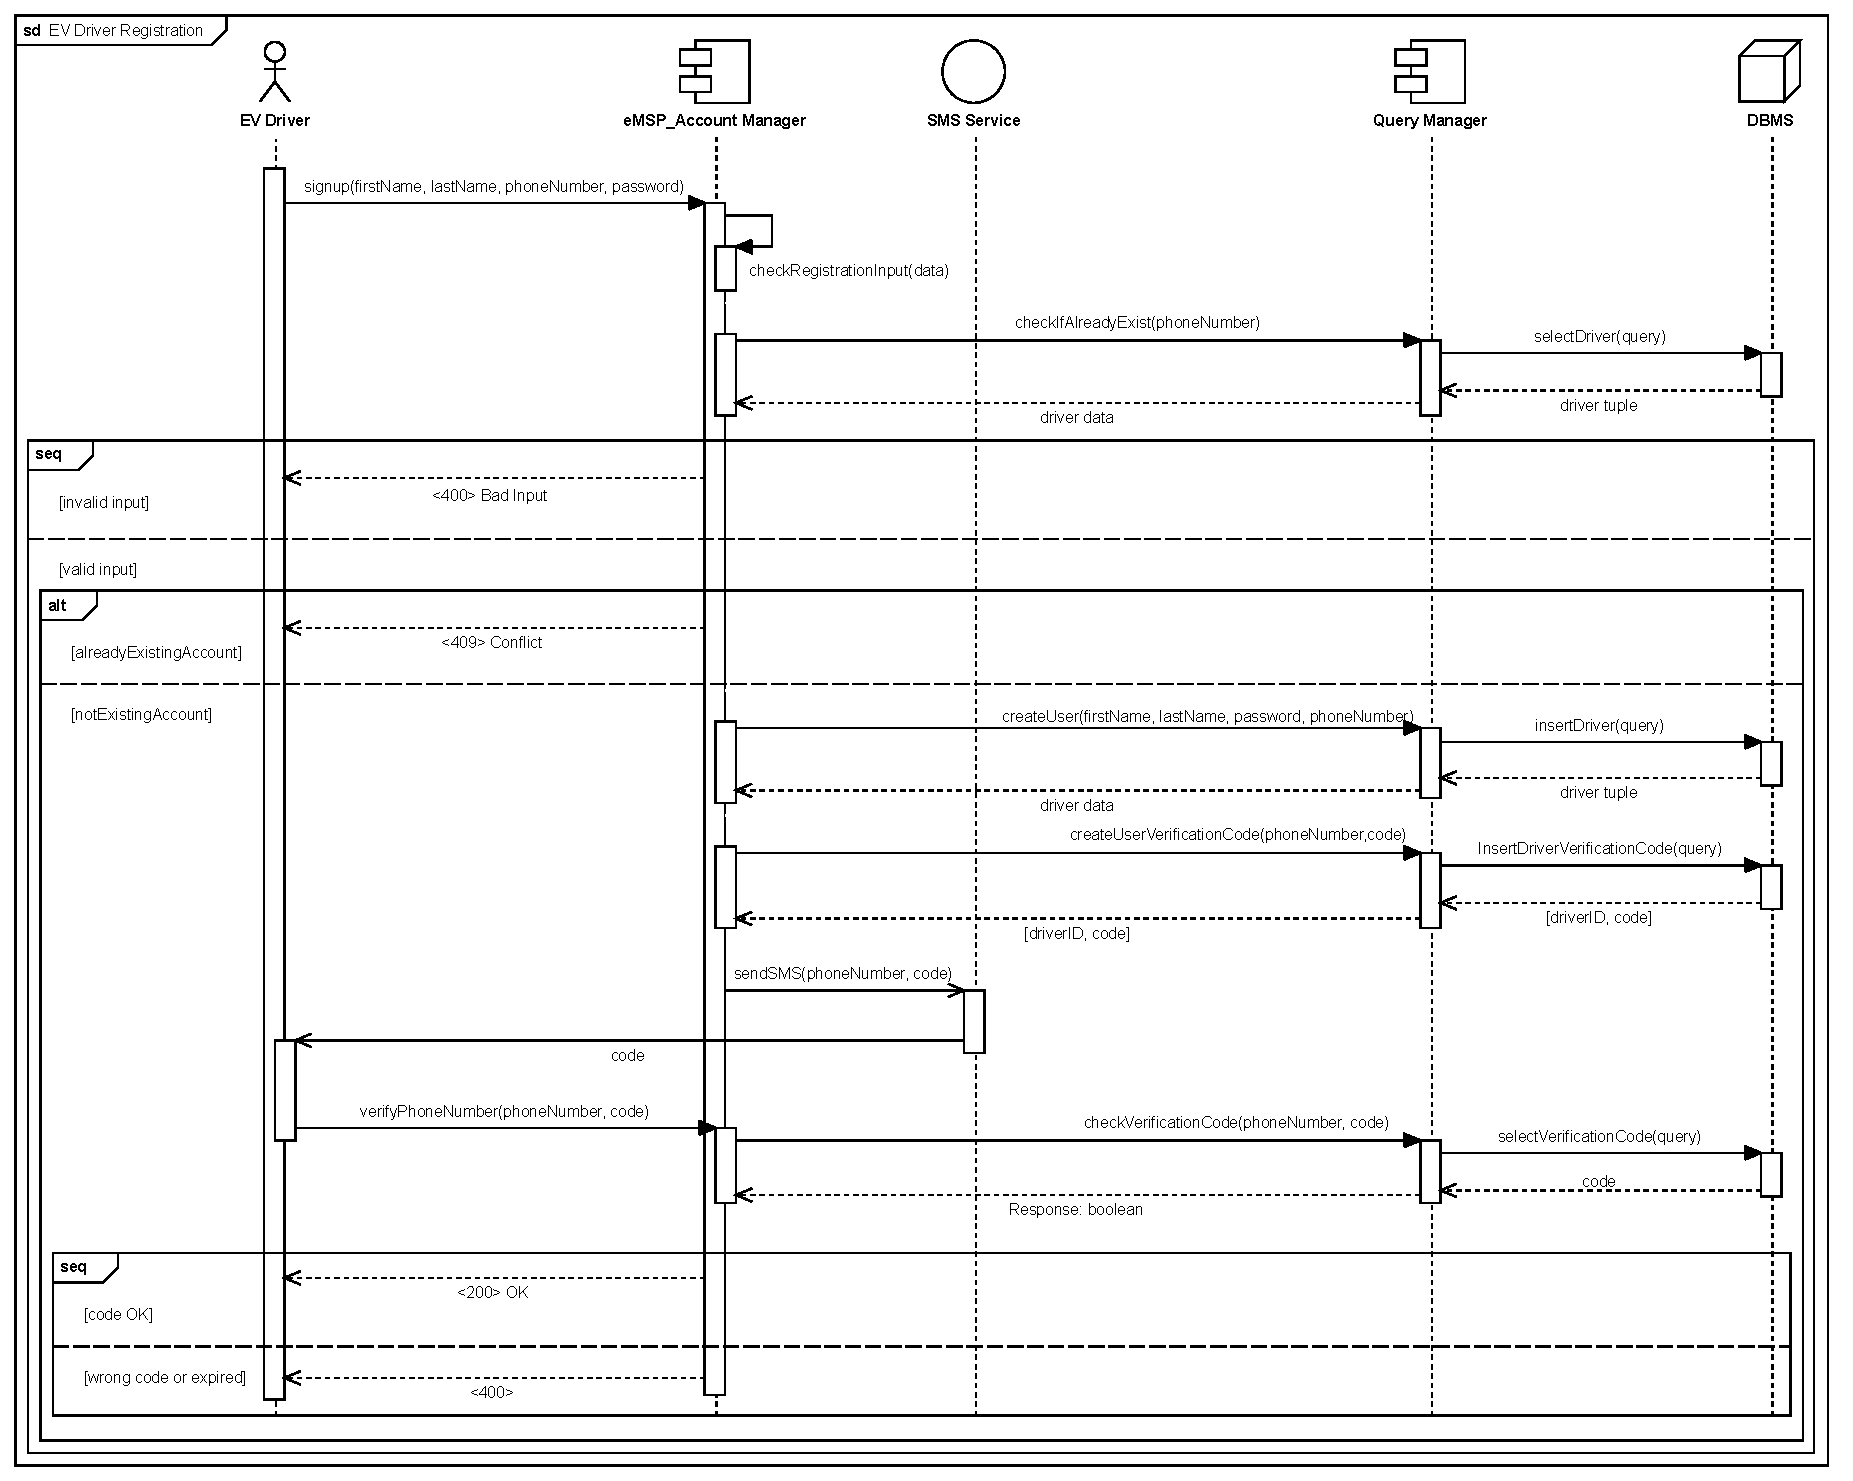
\includegraphics[scale=0.55]{src/runtimeVIew/eMSP_Registration.pdf}
    \caption{EV Driver Registration process}
\end{figure}

\begin{figure}[H]
    \centering
    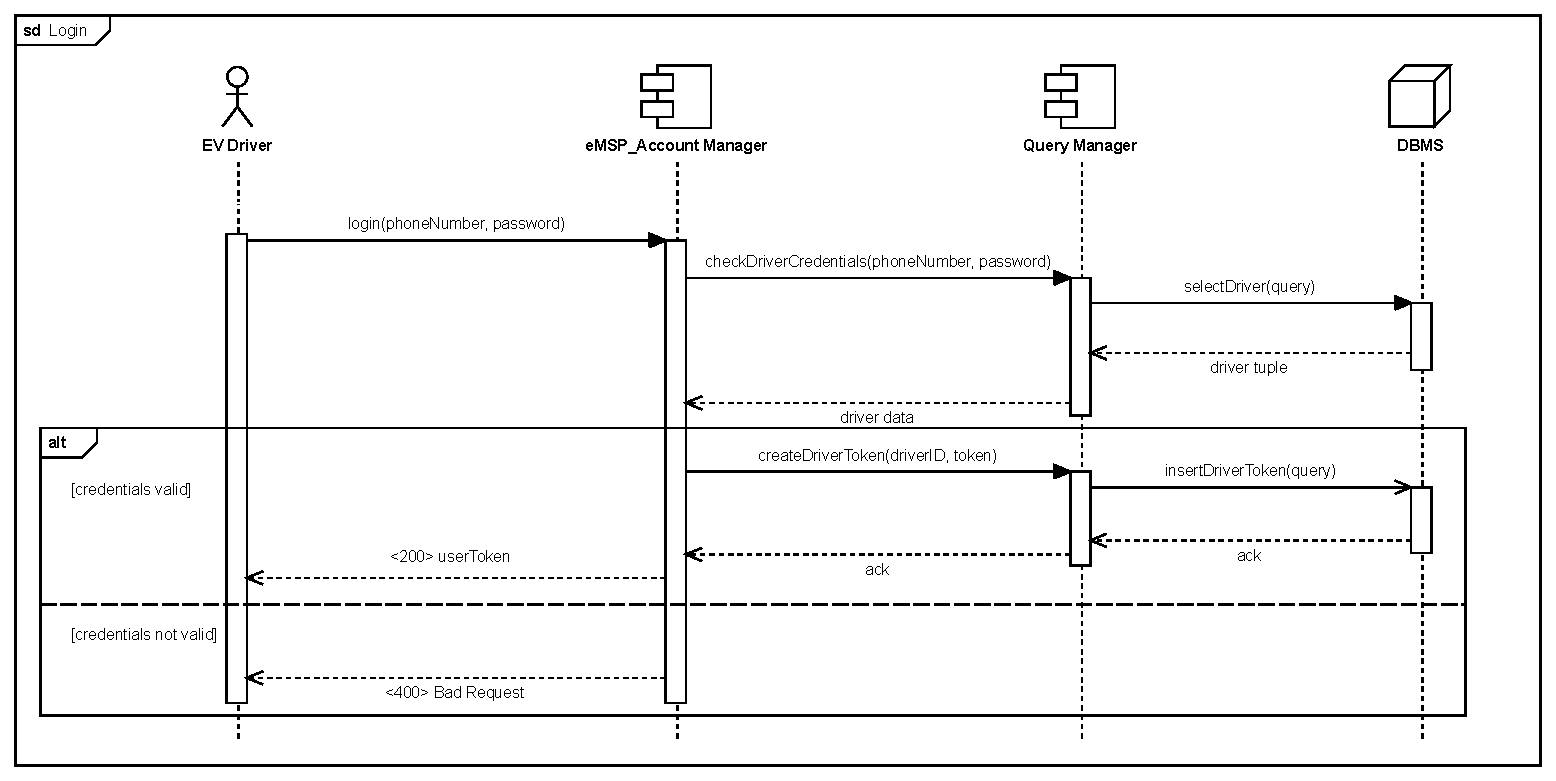
\includegraphics[scale=0.55]{src/runtimeVIew/eMSP_Login.pdf}
    \caption{EV Driver Logs in the system}
\end{figure}

\begin{figure}[H]
    \centering
    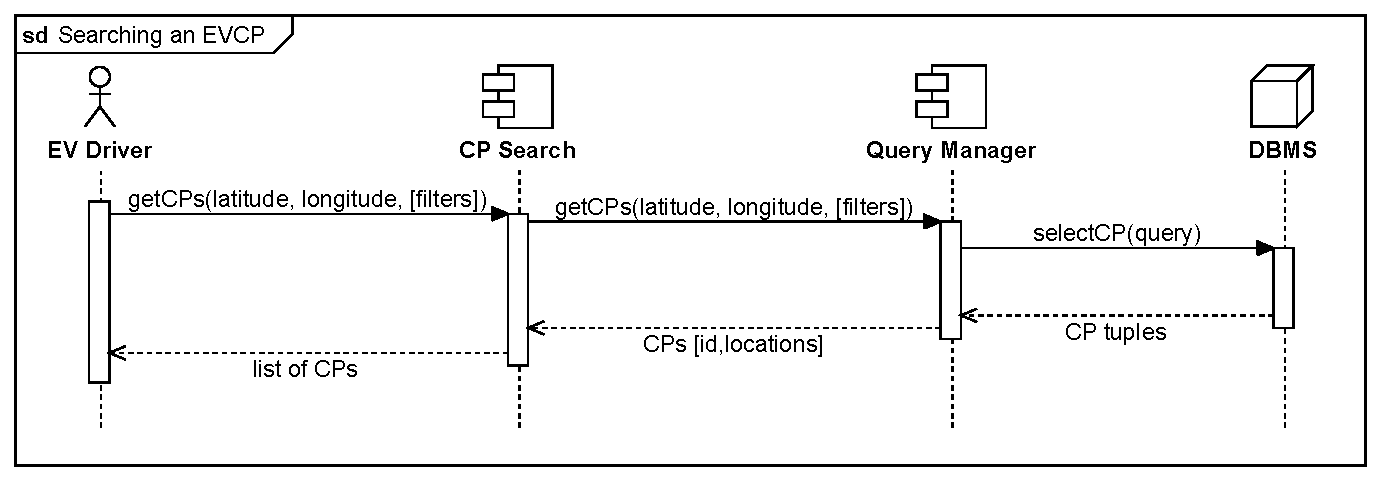
\includegraphics[scale=0.55]{src/runtimeVIew/eMSP_Search.pdf}
    \caption{EV Driver searches on the map}
\end{figure}

\begin{figure}[H]
    \centering
    \hspace*{-2cm}
    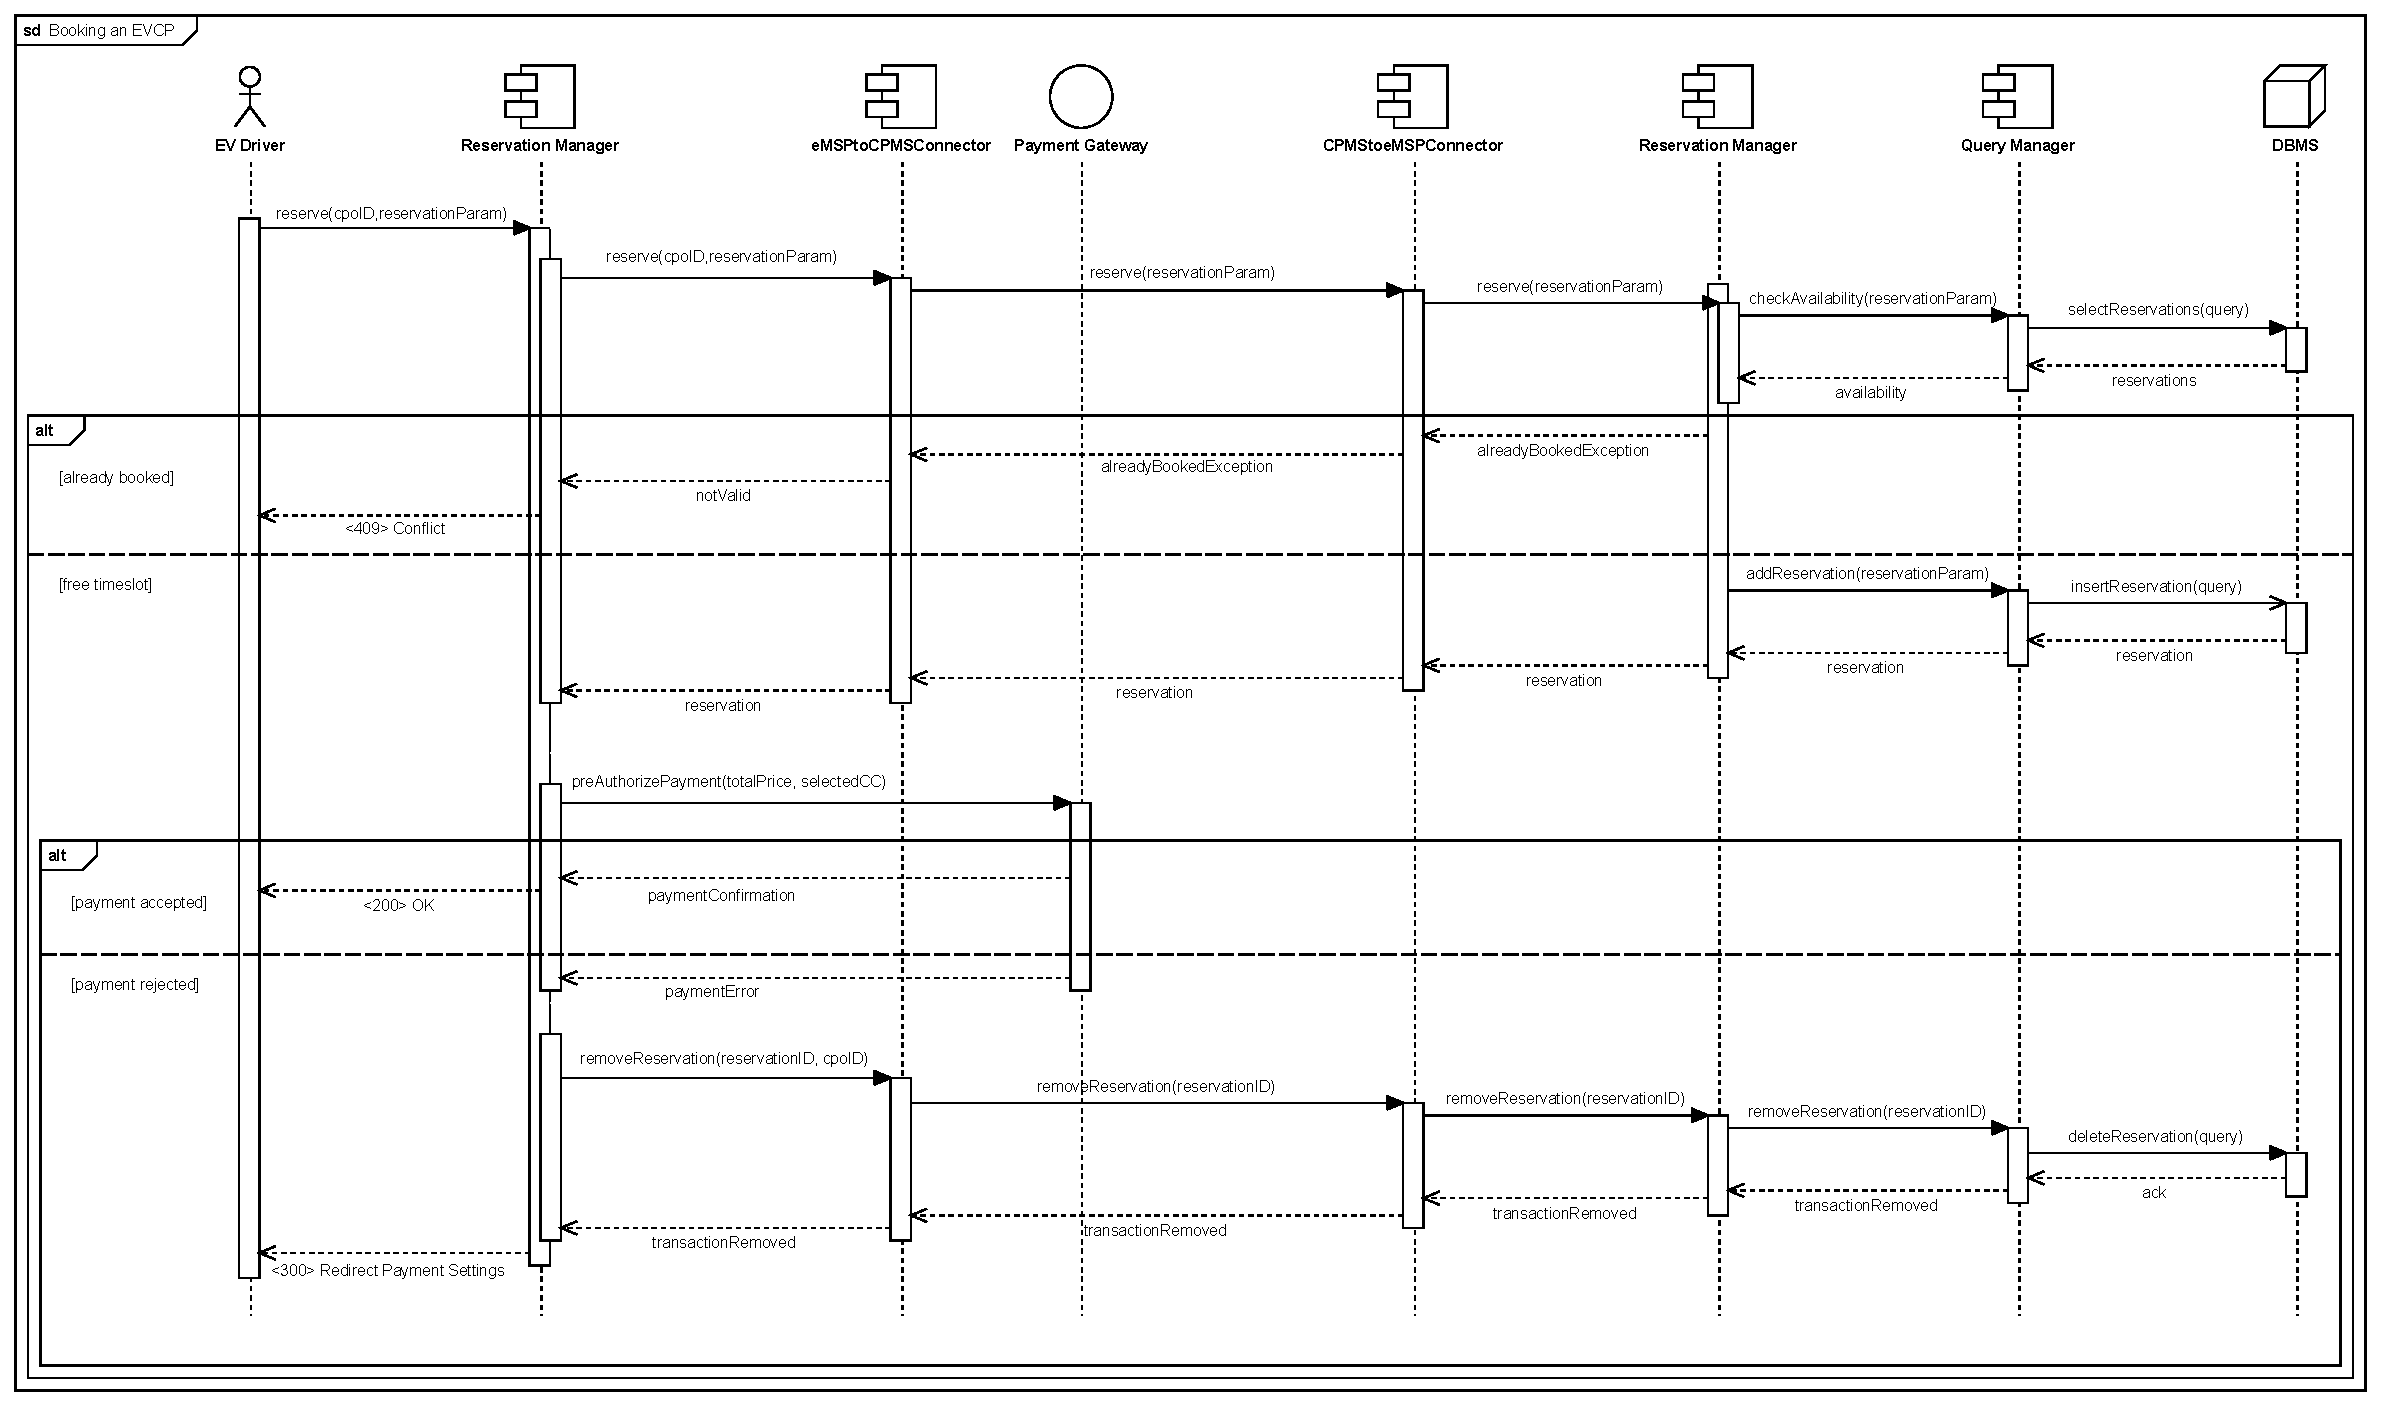
\includegraphics[scale=0.48]{src/runtimeVIew/eMSP_Book.pdf}
    \caption{EV Driver books a charge}
\end{figure}

\begin{figure}[H]
    \centering
    \hspace*{-2cm}
    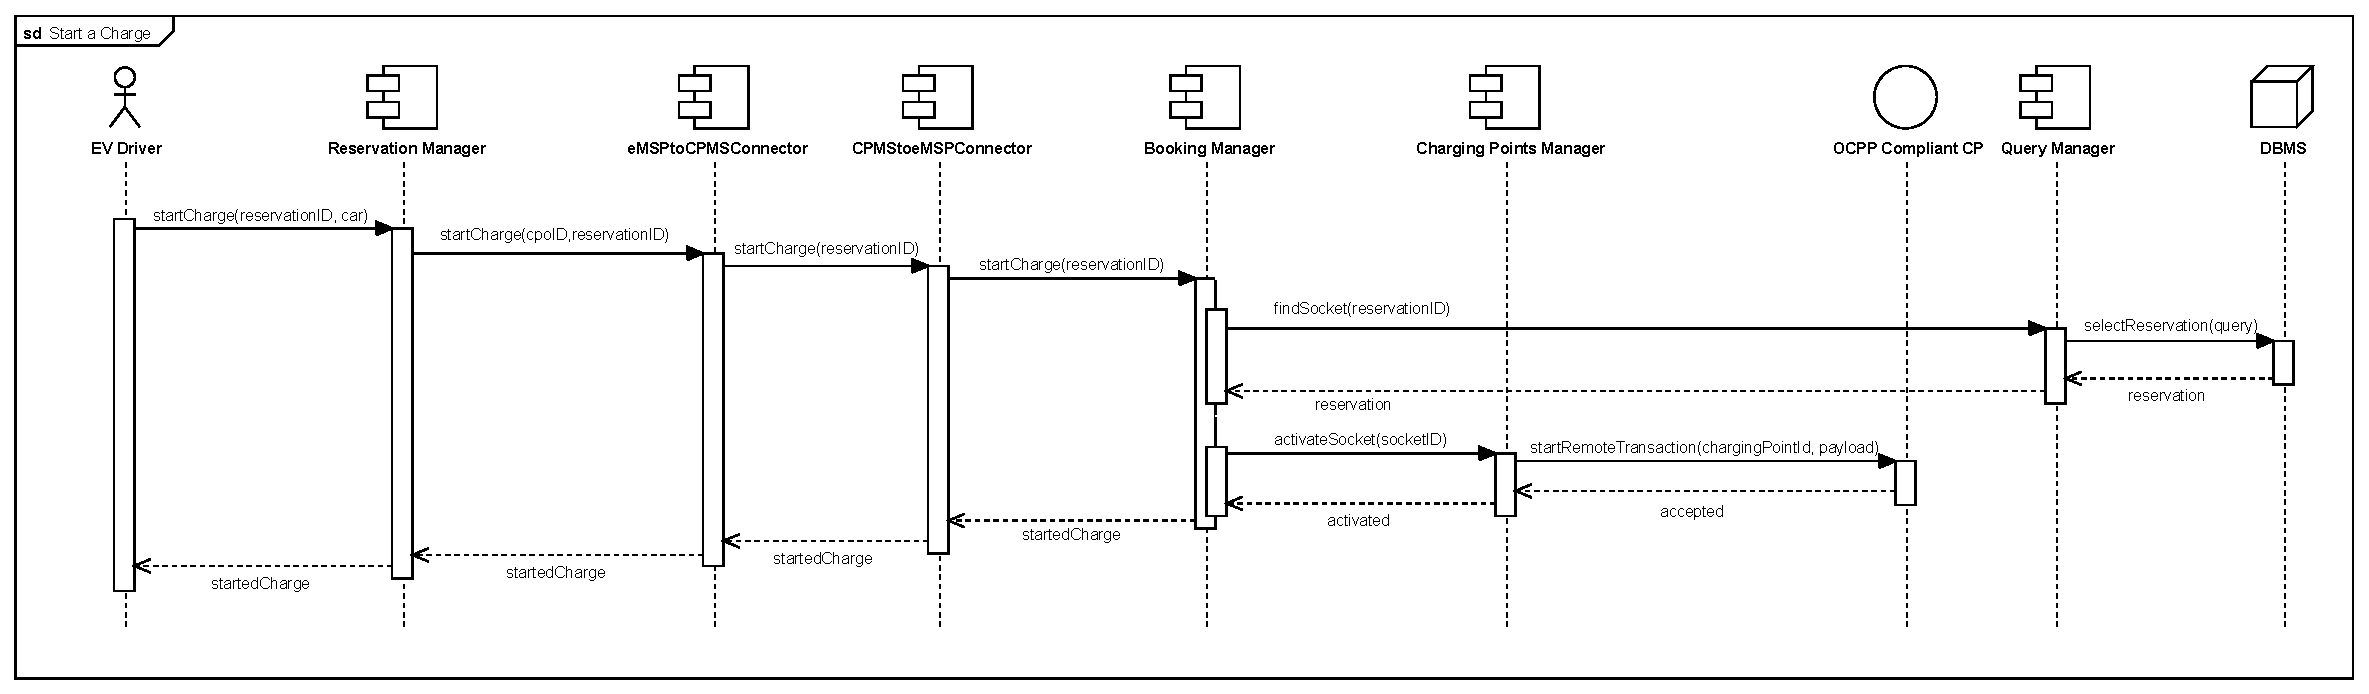
\includegraphics[scale=0.50]{src/runtimeVIew/eMSP_StartACharge.pdf}
    \caption{EV Driver starts a charge}
\end{figure}

\begin{figure}[H]
    \centering
    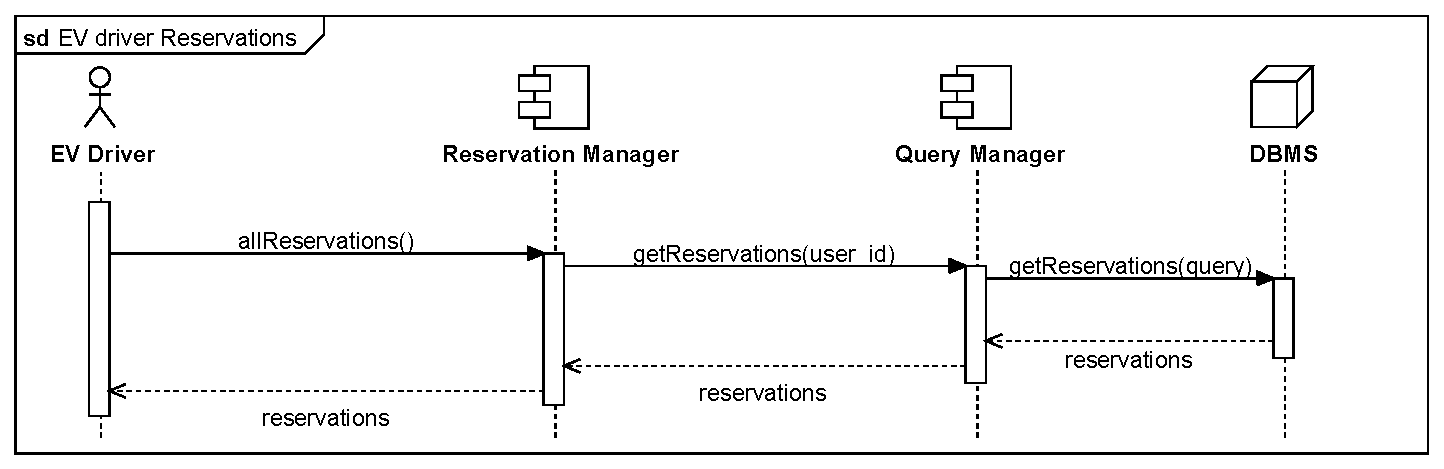
\includegraphics[scale=0.55]{src/runtimeVIew/eMSP_Reservations.pdf}
    \caption{EV Driver sees the reservations}
\end{figure}

\begin{figure}[H]
    \centering
    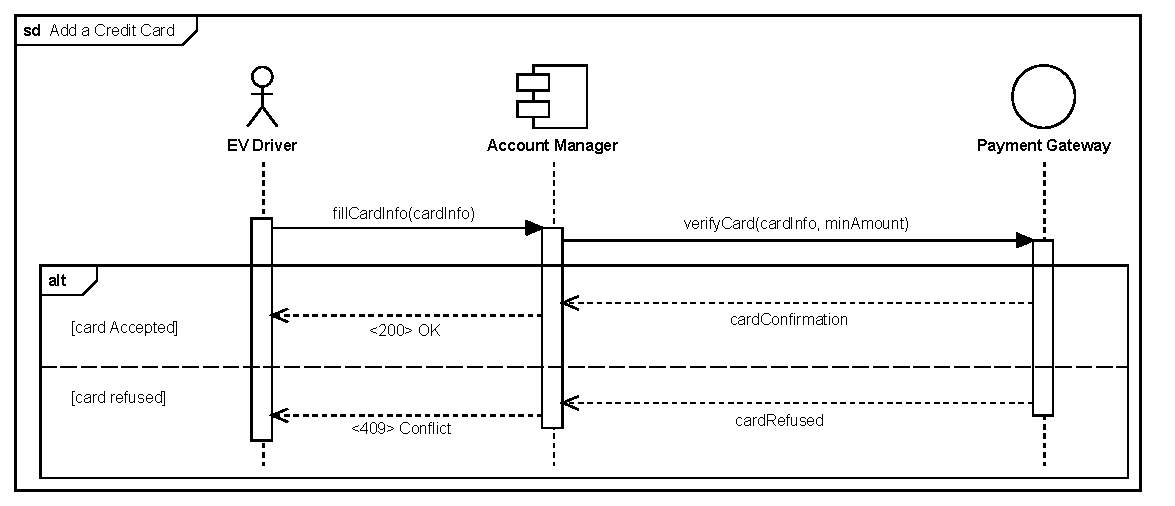
\includegraphics[scale=0.55]{src/runtimeVIew/eMSP_AddCC.pdf}
    \caption{EV Driver adds a credit card information}
\end{figure}

\subsubsection{CPMS}
\begin{figure}[H]
    \centering
    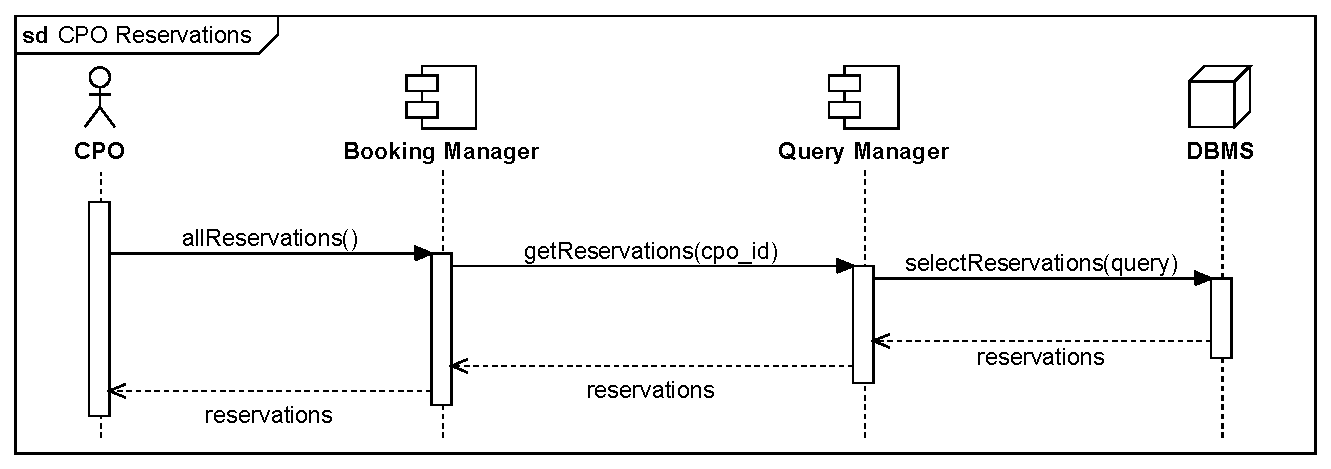
\includegraphics[scale=0.55]{src/runtimeVIew/CPMS_Reservations.pdf}
    \caption{CPO sees the reservations}
\end{figure}

\begin{figure}[H]
    \centering
    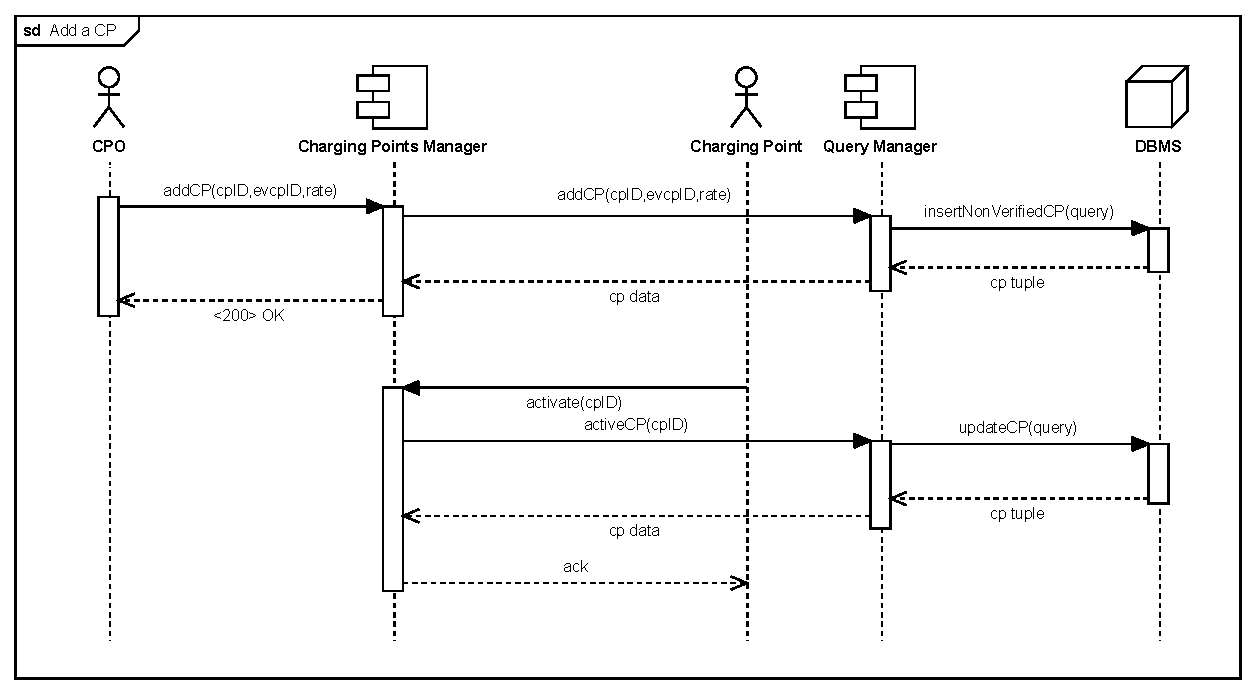
\includegraphics[scale=0.55]{src/runtimeVIew/CPMS_AddCP.pdf}
    \caption{CPO adds a Charging Point}
\end{figure}

\begin{figure}[H]
    \centering
    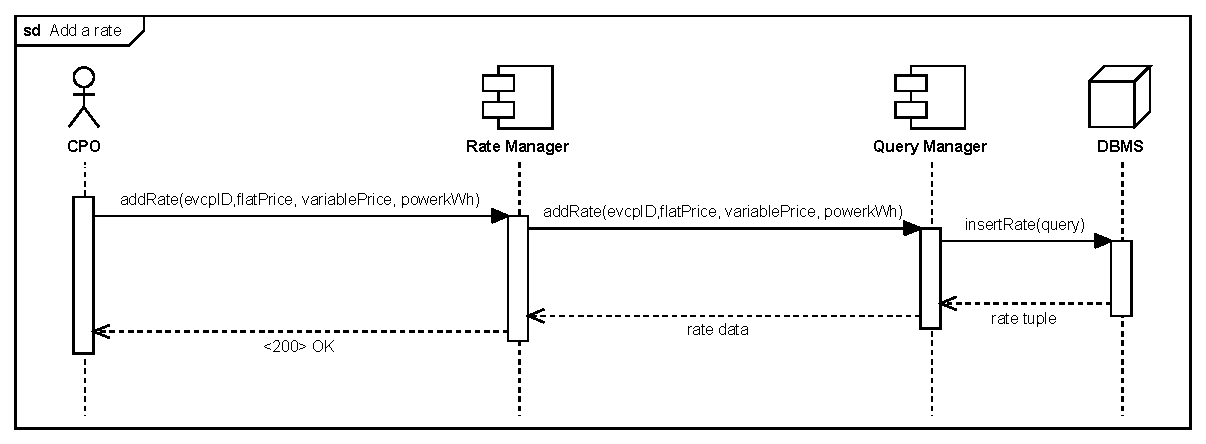
\includegraphics[scale=0.55]{src/runtimeVIew/CPMS_addRate.pdf}
    \caption{CPO adds a rate}
\end{figure}

\begin{figure}[H]
    \centering
    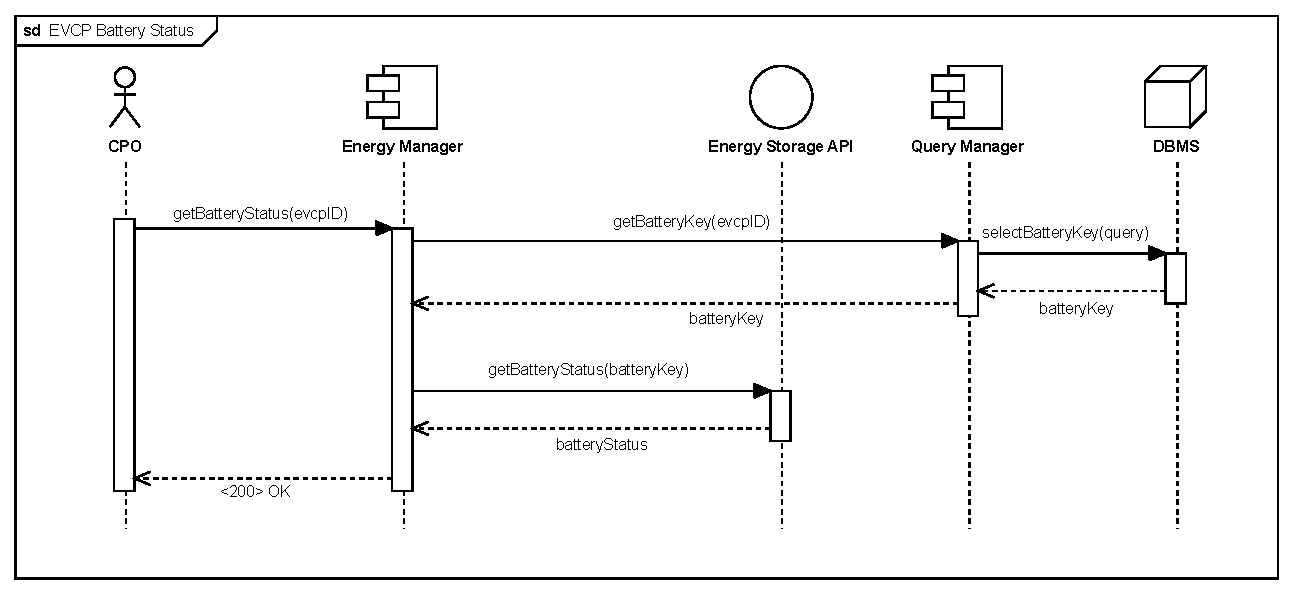
\includegraphics[scale=0.55]{src/runtimeVIew/CPMS_batteryCapacity.pdf}
    \caption{CPO sees the battery capacity}
\end{figure}

\begin{figure}[H]
    \centering
    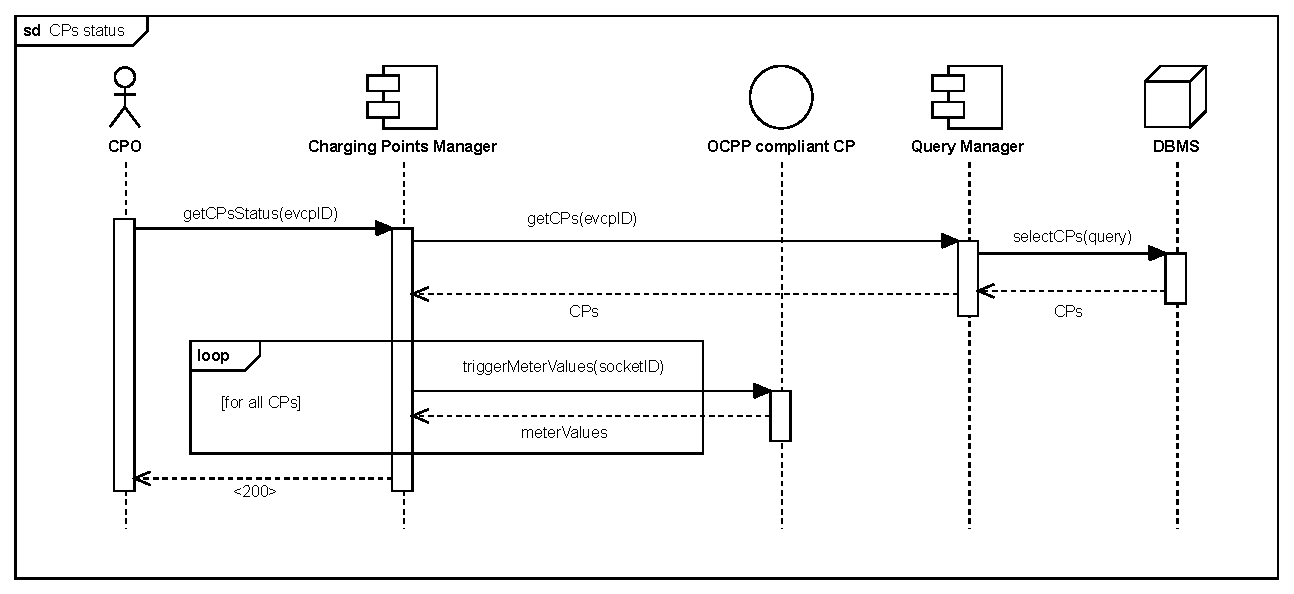
\includegraphics[scale=0.55]{src/runtimeVIew/CPMS_CPsStatus.pdf}
    \caption{CPO sees the status of its Charging Points}
\end{figure}

\begin{figure}[H]
    \centering
    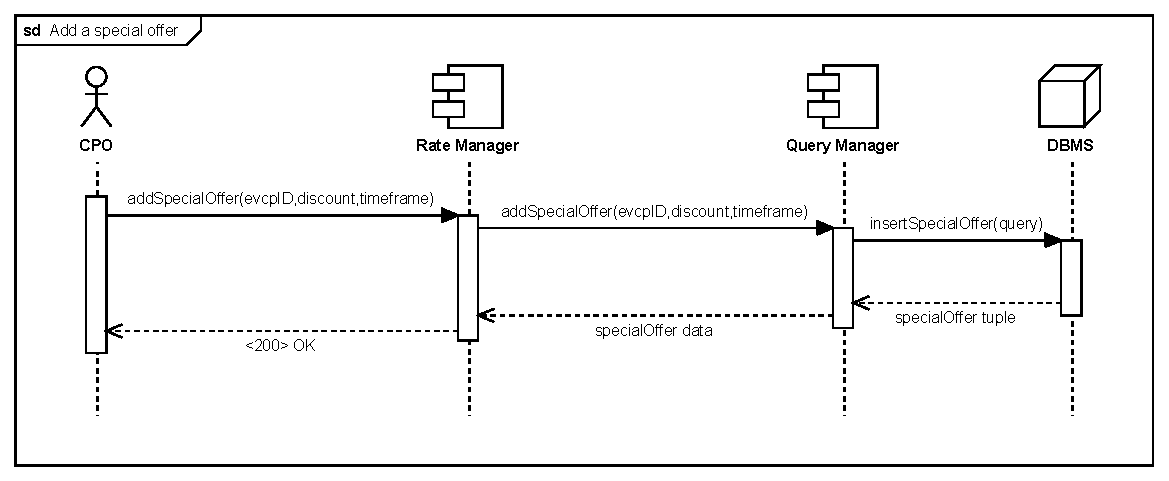
\includegraphics[scale=0.55]{src/runtimeVIew/CPMS_specialOffer.pdf}
    \caption{CPO adds a special offer}
\end{figure}

\subsection{Component interfaces}
Details for each interface (name, signature, returned objects)
\subsubsection{REST Endpoints}
\renewcommand{\labelitemii}{}
\renewcommand{\labelitemiii}{-}
\begin{itemize}
    \item \texttt{/api/search/<latitude|longitude>}
          \begin{itemize}
              \item Maps: \texttt{NomeMetodoMappato}
              \item Type: TipoAPI(GET,POST)
              \item URL Parameters:
                    \begin{itemize}
                        \item \texttt{<latitude|longitude>} - GPS Location, needed to find CPs nearby a certain location.
                    \end{itemize}
              \item Parameters:
                    \begin{itemize}
                        \item \texttt{authToken}
                        \item \texttt{blabla} [string] - description
                        \item \texttt{blabla} [boolean] - description
                        \item \texttt{blabla} [number] - description
                    \end{itemize}
              \item Success:
                    \begin{itemize}
                        \item 200 - OK + Response
                              \begin{lstlisting}
            {
                "cps": [
                    {
                        "id": "<store id>",
                        "name": "<cp name>",
                        "address": "<address>",
                        "open": <boolean>,
                        "distance": <number>,
                    }
                ]
            }
            \end{lstlisting}
                    \end{itemize}
              \item Errors:
                    \begin{itemize}
                        \item 400 - Bad request
                        \item 404 - No store found
                    \end{itemize}
          \end{itemize}
\end{itemize}

\subsection{Architectural Styles and patterns}
Please explain which styles/patterns you used, why, and how

\begin{itemize}
    \item Three layers and Four Tier: what and why?
    \item RESTful: what and why?
    \item Adapter Pattern: The Query Manager component implements the Adapter pattern, as it mediates between the
          business logic and the DBMS services, exposing only a restricted and higher level set of functionalities.
\end{itemize}
\subsection{Other design decisions}
\subsubsection{PWA}
\dots
\subsubsection{Scale-out}
\dots
\subsubsection{Relational Database}
\dots
\subsubsection{The separation of eMSP and CPMSs}
\section{User Interface Design}
In RASD we already did mockups so here we put UX flowcharts.
Overview of UIs, possibly mockups, may refine what’s in the RASD (if present)

\begin{figure}[H]
    \centering
    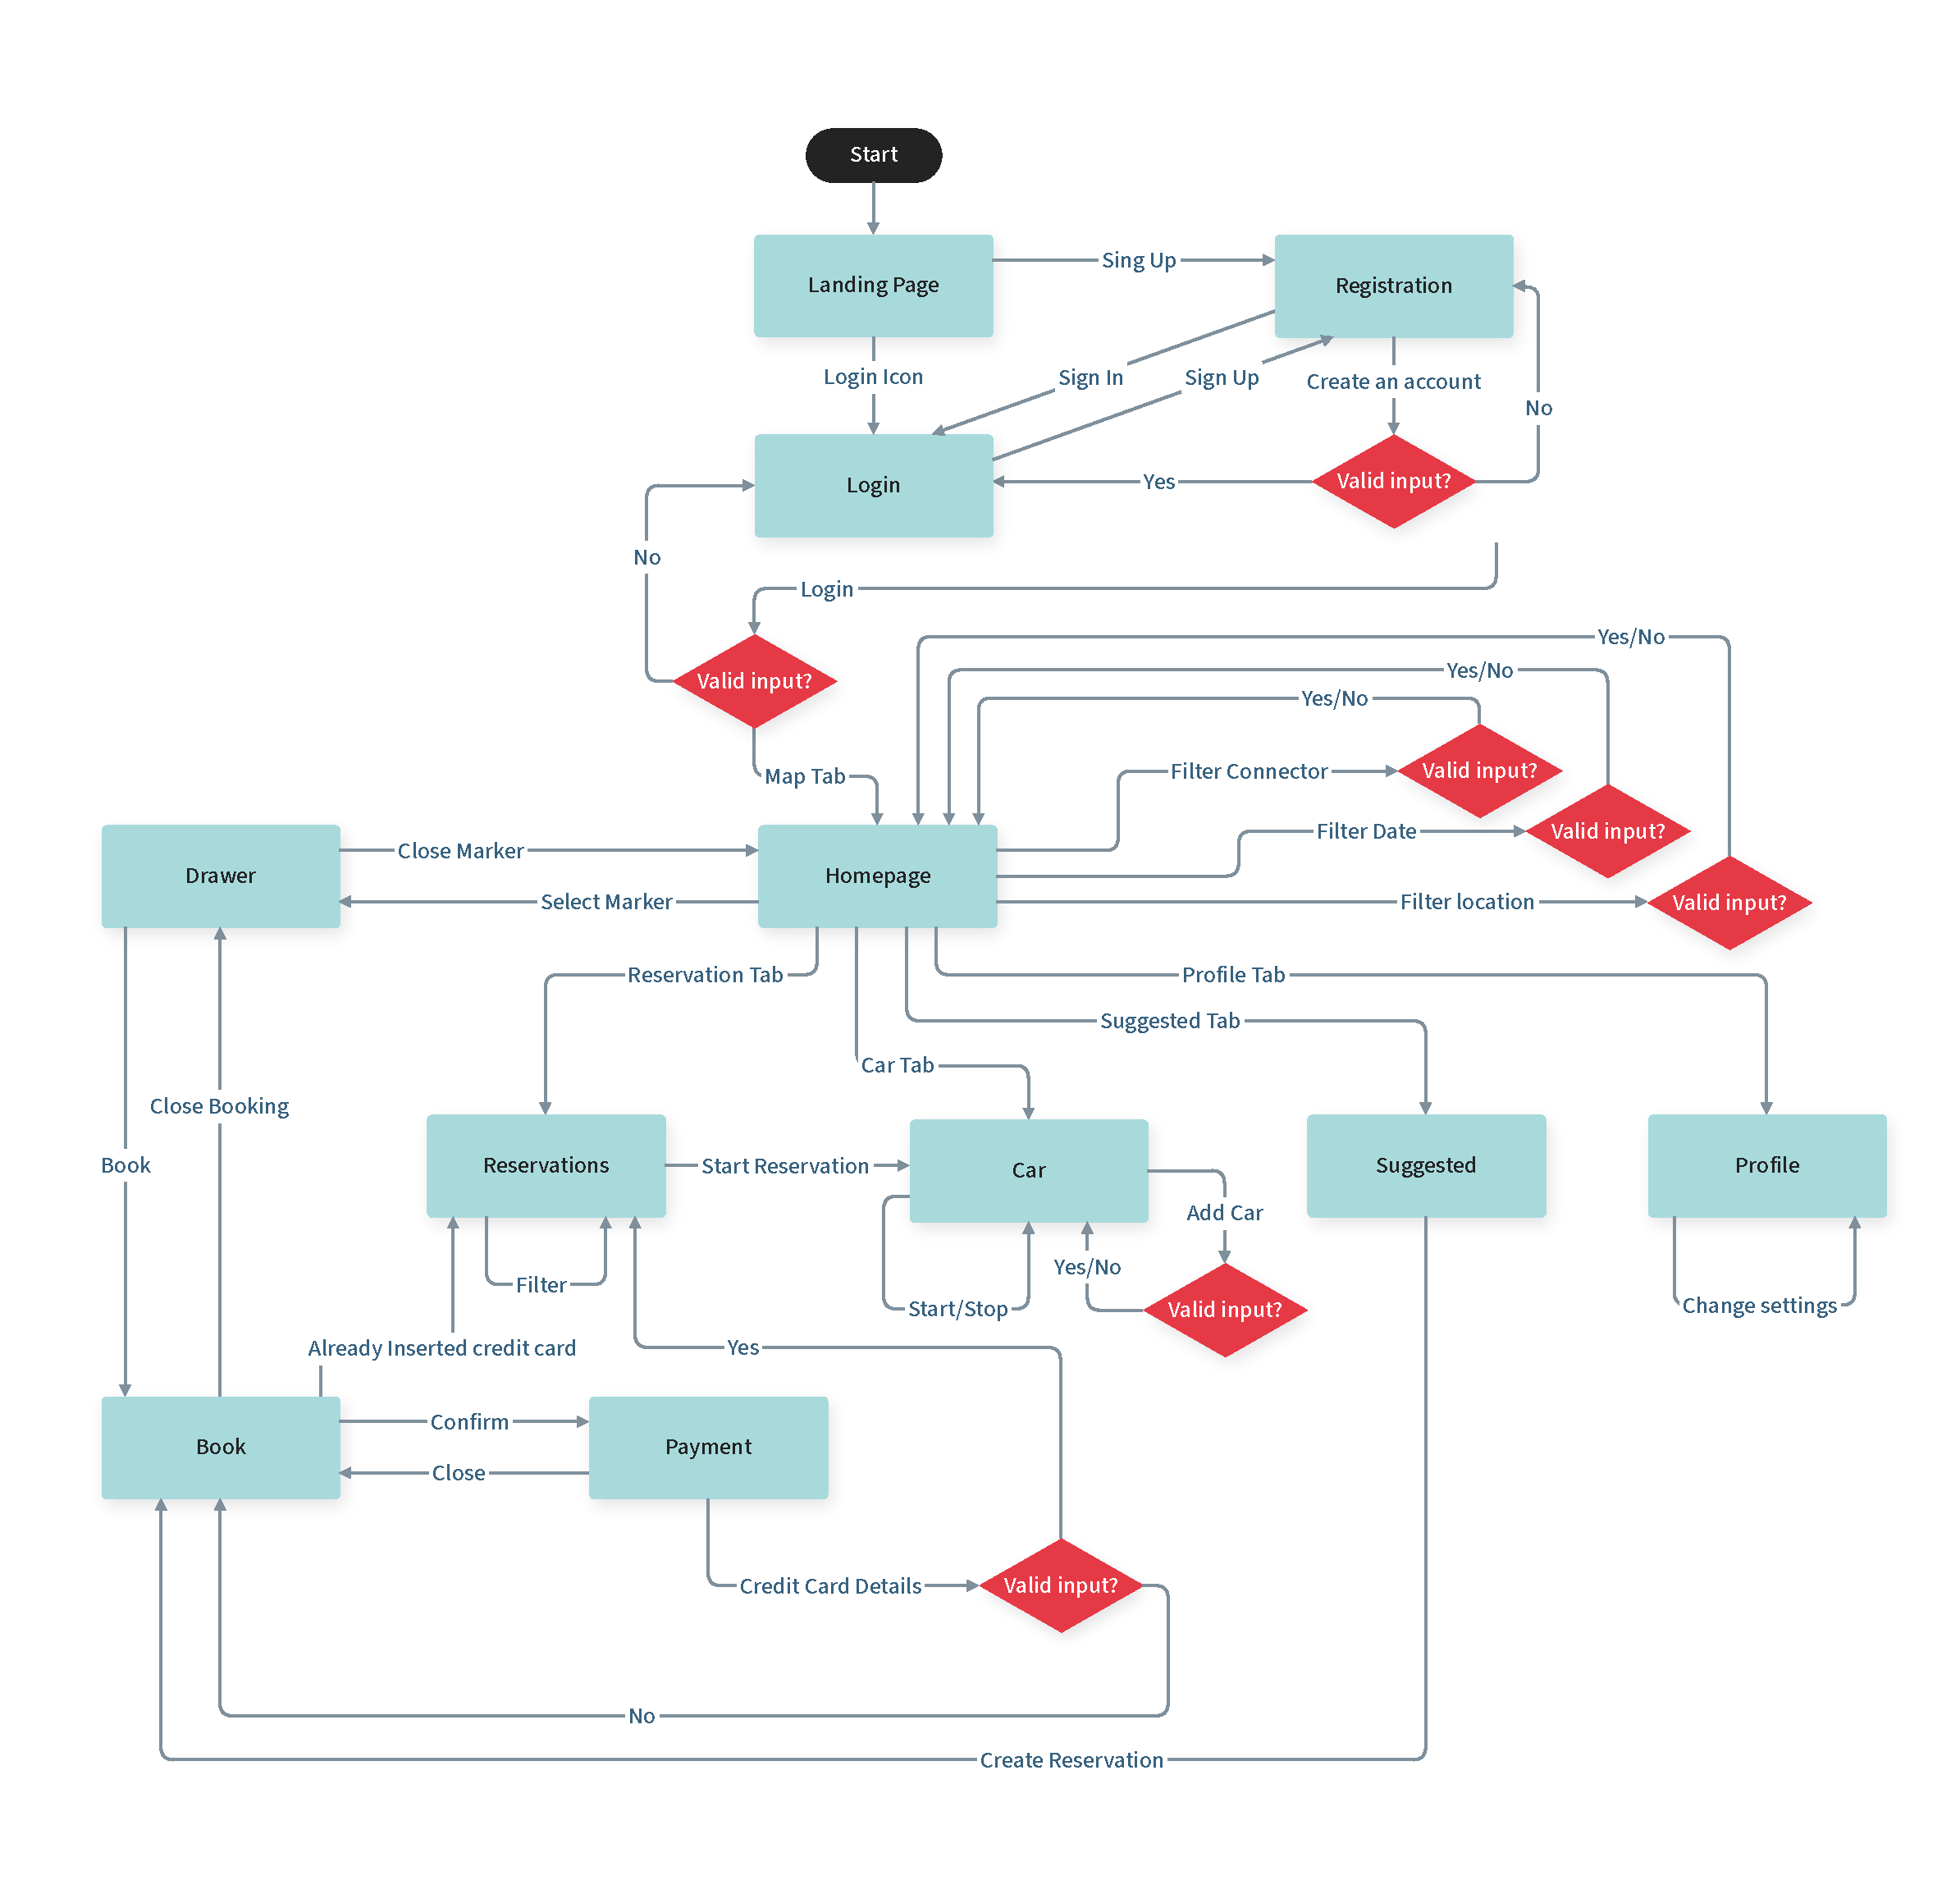
\includegraphics[scale=0.41]{src/UIDesign/User.pdf}
    \caption{EVdriver}
\end{figure} \vspace{1cm}

\begin{figure}[H]
    \centering
    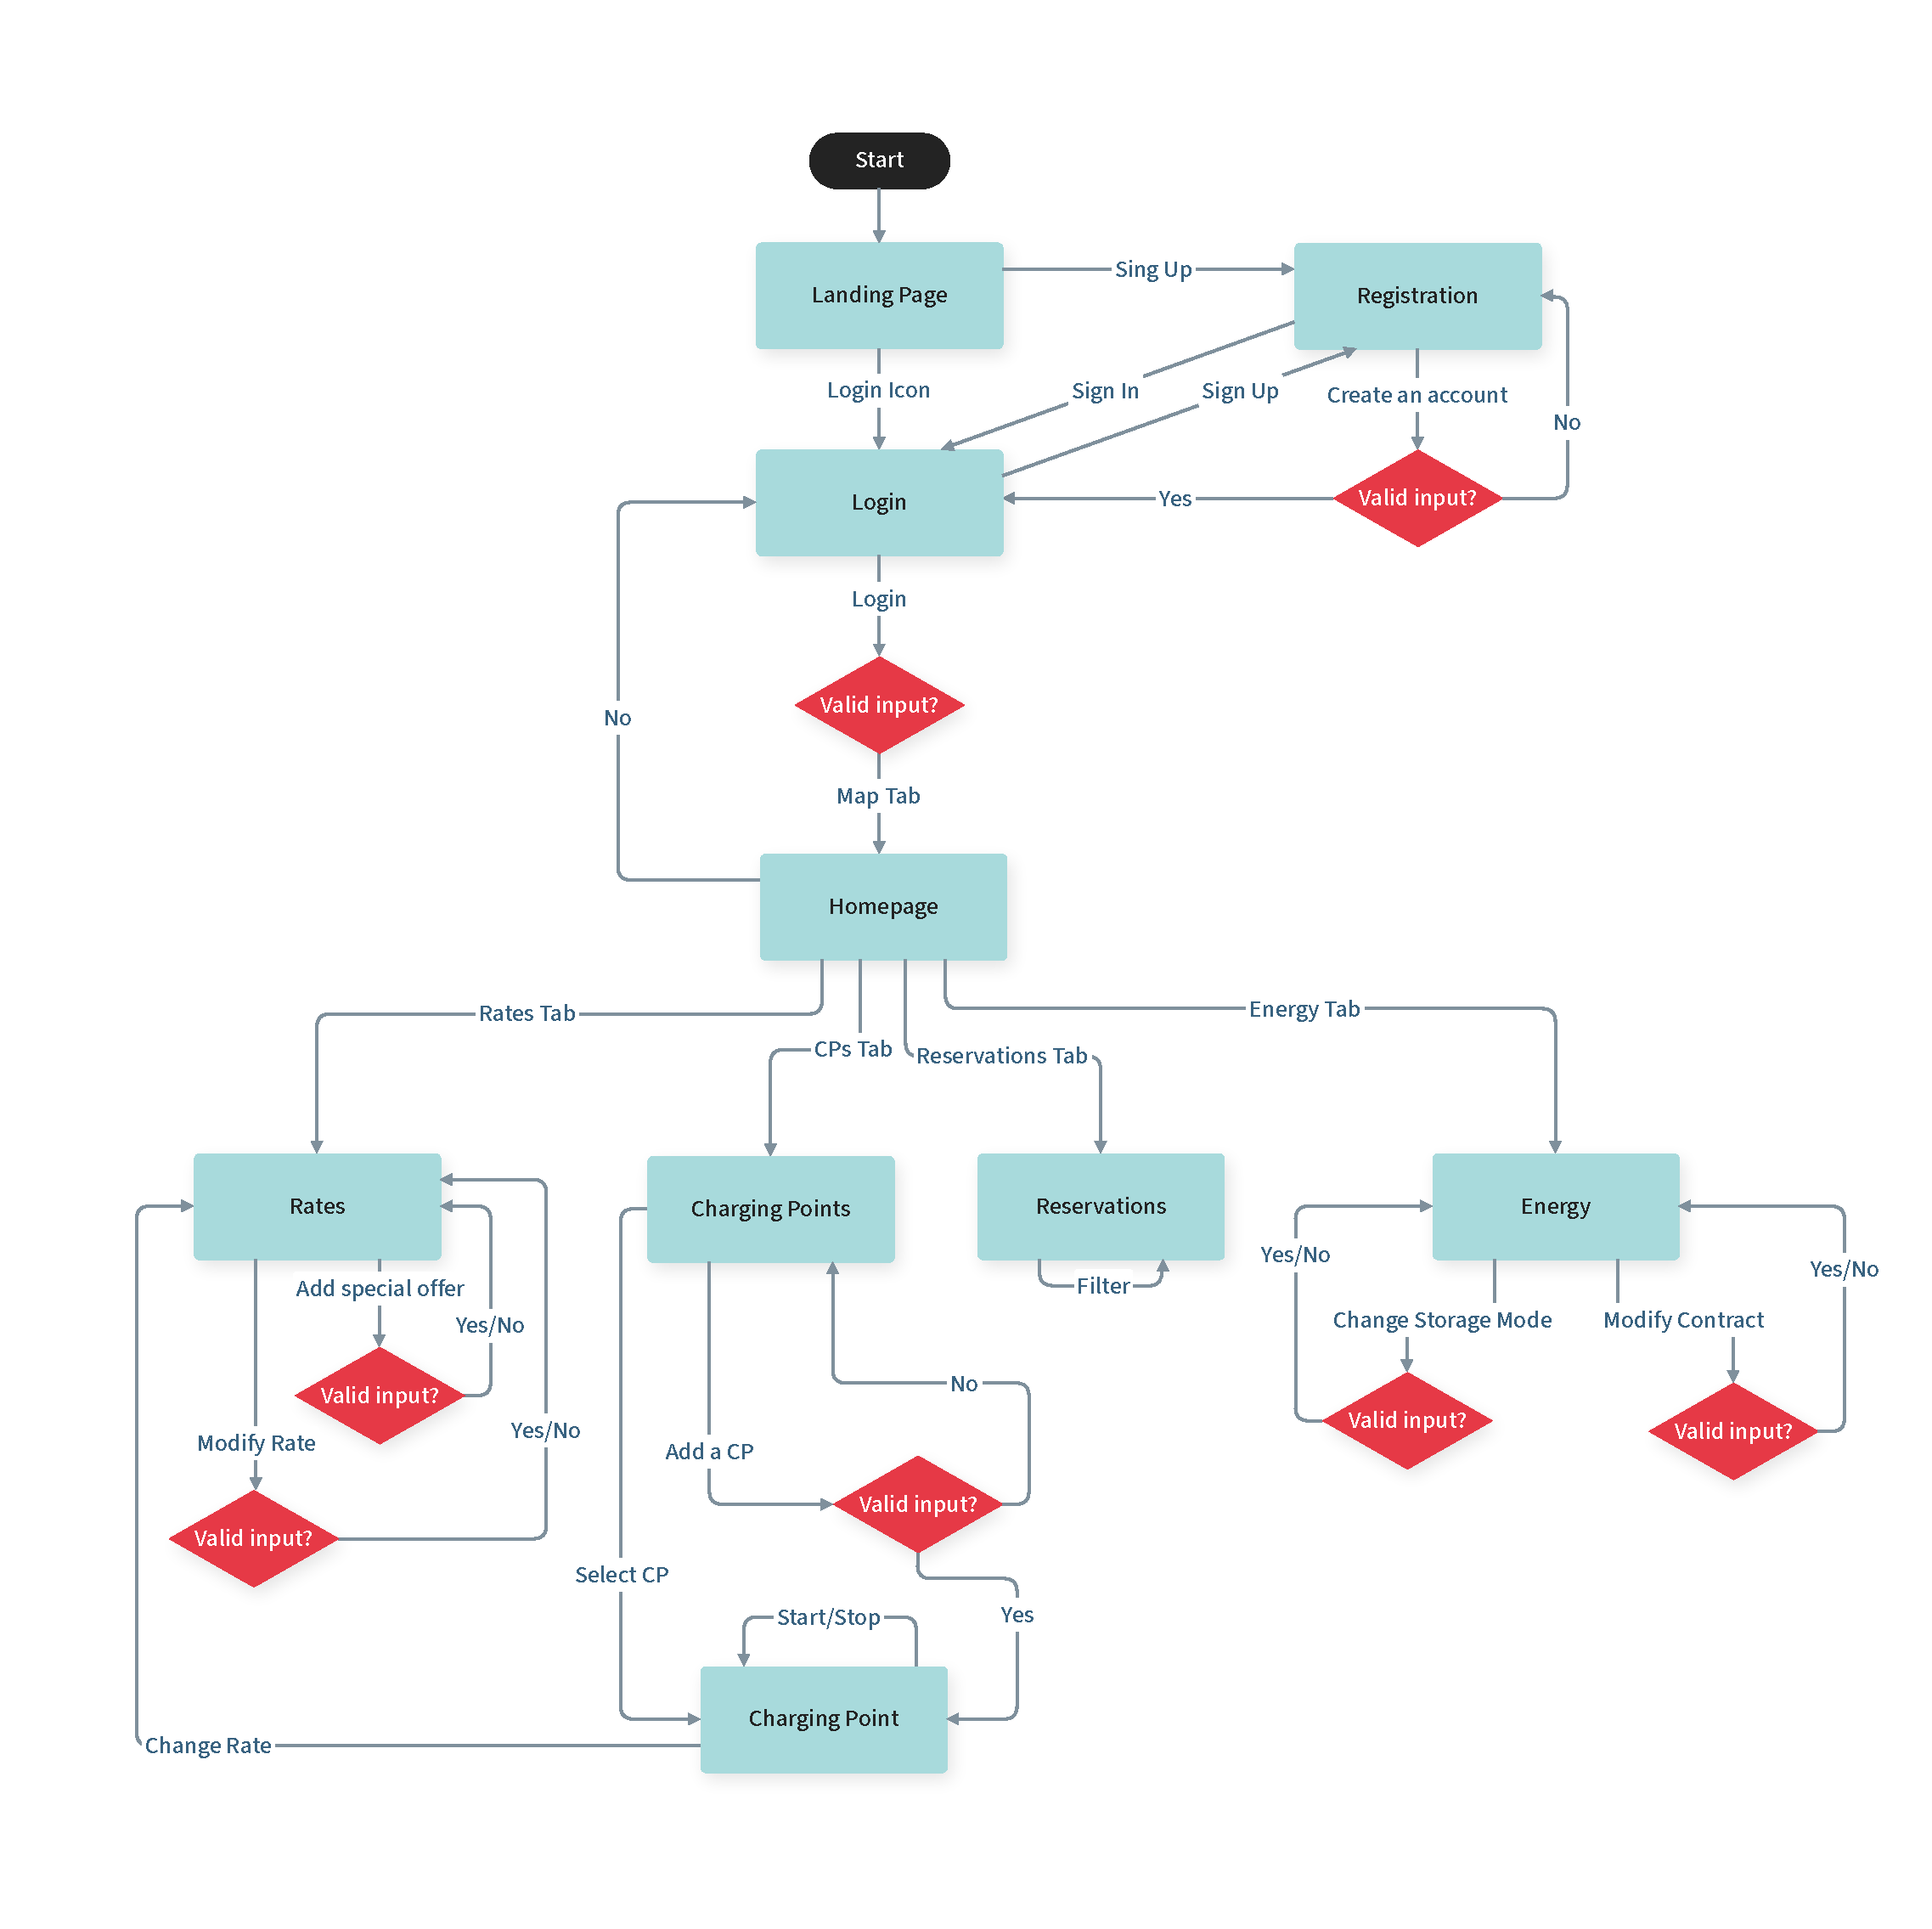
\includegraphics[scale=0.41]{src/UIDesign/Cpo.pdf}
    \caption{Charging Point Operator}
\end{figure} \vspace{1cm}
\section{Requirements traceability}
Mapping between requirements and components
Explain how the requirements you have defined in the RASD map to the design elements that you have defined in this document.
\section{Implementation, integration and testing plan}
This section will be dedicated to discuss how the subcomponents' implementation is planned, to present the integration plan and then
to explain the tests dedicated to evaluate if the System behaviours as expected. 
\subsection{Development Process and Approach}
The application is composed of three layers (client, business and data) and these layers can be implemented in parallel and integrated.
The tiers can be unit tested independently and after the integration they can be tested at the end as the whole System.
The whole System can be implemented, integrated and tested exploiting bottom-up approach. The decision to use this approach derives
from the possibility to incrementally develop the system by proceeding implementing in parallel the different tiers. 
The components are tested and integrated with other components to evaluate the dependencies between components of the same subsystem.

\subsubsection{Frontend}
It consists of the PWA and web application for the EV Drivers and the web application for CPOs that can be developed and tested independently
since are decoupled and doesn't communicate directly. Both the two components rely on REST API to interact with the business logic and can be unit tested by mocking 
the REST APIs. 
\subsubsection{Backend}
It consists of business logic and the data logic. The application server of the business logic is composed by the Query Manager and two important components,
the eMSP and the CPMS that need to communicate each other. The developers can be work separately on 
eMSP and CPMS and integrate and test at the end of their development the two components to evaluate the dependency and the interactions between them.
These whole business logic can be tested independently from the client logic, speeding up the development process. 
In the following two sections will be analyzed the complexity and the importance for the subcomponents of the eMSP and the CPMS.
\\
\begin{itemize}
    \item \textbf{eMSP} \\ In the following two sections will be analyzed the complexity and the importance for the subcomponents of the eMSP.
    
    \begin{center}
        \begin{tabular}{|p{6cm}|l|l|}
            \hline
            \textbf{Component} & \textbf{Importance} & \textbf{Complexity}\\
            \hline
            Account Manager & High & Medium \\
            \hline
            CP Search Manager & High & Medium \\
            \hline
            Car Manager & Medium & Medium \\
            \hline
            Reservation Manager & High & High \\
            \hline
            Suggestion Manager & Medium & Medium \\
            \hline
            Notification Manager & Medium & Medium \\
            \hline
            eMSPtoCPMSConnector & High & High \\
            \hline
            Query Manager & High & Low \\
            \hline
         \end{tabular}
    \end{center}
    \noindent \\
    \item \textbf{CPMS} \\ In the following two sections will be analyzed the complexity and the importance for the subcomponents of the CPMS.
    
    \begin{center}
        \begin{tabular}{|p{6cm}|l|l|}
            \hline
            \textbf{Component} & \textbf{Importance} & \textbf{Complexity}\\
            \hline
            Account Manager & High & Medium \\
            \hline
            Rate Manager & Medium & Low \\
            \hline
            Energy Manager & Medium & Medium \\
            \hline
            Booking Manager & High & High \\
            \hline
            Charging Points Manager & High & High \\
            \hline
            Query Manager & High & Low \\
            \hline
         \end{tabular}
    \end{center}
    \noindent \\
\end{itemize}

\subsubsection{External components} 
All the external APIs are provided by third parties and are supposed to be reliable and conform to their specification. 

\subsection{Implementation Plan}
The implementation of the Application Server will be divided between eMSP and CPMS a can be done in parallel.
\subsubsection{eMSP}
\begin{enumerate}
    \item \textbf{Query Manager}: It is the first component to be implemented since all the other component relies on This
    on to interact with the Database. It is the only component in which is necessary to implement the queries to the database.
    \item \textbf{Notification Manager}: Then component can be implemented, it offers two interfaces to two components that will later 
    be developed.
    \item \textbf{eMSP's account Manager}: This is the component that permits to register or log in a user. It has an authorization interface that 
    is used by the other components to verify at each request that the user has the permissions to do the requested operations.
    \item \textbf{eMSPtoCPMSConnector}: The development of this module is particularly critic because is the component dedicated
    to the communication with the CPMS. The dialogue between the two can be simulated during the implementation and tested after the integration.
    \item \textbf{Charging Points Manager, Reservation Manager, Suggestion Manager, Car Manager}: These components can be implemented
    in parallel since there are no dependencies between them. 
\end{enumerate}
\subsubsection{CPMS}
\begin{enumerate}
    \item \textbf{Query Manager}: It is the first component to be implemented since all the other component relies on This
    on to interact with the Database. It is the only component in which is necessary to implement the queries to the database.
    \item \textbf{CPMS's account Manager}: This is the component that permits to register or log in a user. It has an authorization interface that 
    is used by the other components to verify at each request that the user has the permissions to do the requested operations.
    \item \textbf{CPMStoeMSPConnector}: The development of this module is particularly critic because is the component dedicated
    to the communication with the eMSP. The dialogue between the two can be simulated during the implementation and tested after the integration.
    \item \textbf{Rate Manager}: This component has to be implemented before the Charging Points Manager because during the adding 
    of a new CP to the Manager, a rate needs to be associated to the CP.
    \item \textbf{Charging Points Manager and Booking Manager}: These two components are the most critical to implement but also two 
    of the most essential components. The dialogue between the CPMS and the CPs is done through the Charging Points Manager that 
    needs to be implemented compliant with the OCPP protocol used by the CPs. The Reservation Manager on the other hand is the component
    that manages all the reservation done through the eMSP to the specific CPMS. These two components can be implemented in parallel.
    \item \textbf{Energy Manager}: This component has a medium complexity because it interacts with the DSO Pricing Service and Energy Storage API. 
\end{enumerate}

\subsection{Integration Plan}
The section describes the integration plan of the different components and subcomponents of the eMAll System. 
The graphs below show the dependencies of a component or subcomponent on another component or subcomponent. Each subcomponent before being integrated with others subcomponents
to form a component need to be unit tested and after the integration the integrated component will be tested.
The testing can be done in parallel between eMSP and CPMS.
\subsubsection{eMSP}
The first components to be tested together are the Query Manager and the DBMS as they are the components necessary for all the others when handling data.
\begin{figure}[H]
    \centering
    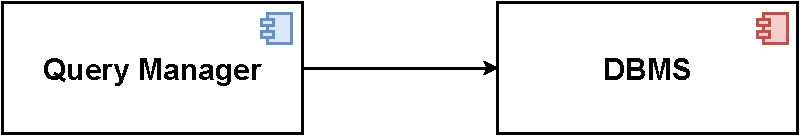
\includegraphics[scale=0.6]{src/Integration/eMSPQuery.pdf}
    \caption{Data Subsystem}
\end{figure}
Before implementing the Account Manager it is preferred to develop the Notification Manager.
\begin{figure}[H]
    \centering
    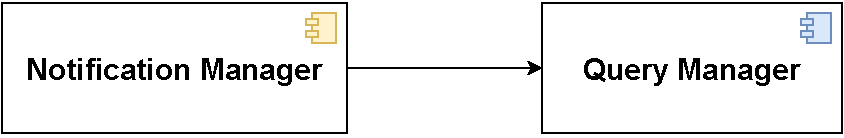
\includegraphics[scale=0.6]{src/Integration/eMSPNotification.pdf}
    \caption{Notification Subsystem}
\end{figure}
Then it can be implemented the Account Manager that provides the account managing functions and the authorization interface 
to verify the permissions to do operations with the other components. It handles personal user's data and for this reason needs
to be tested carefully.
\begin{figure}[H]
    \centering
    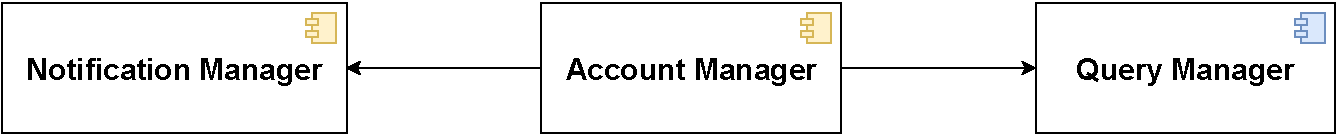
\includegraphics[scale=0.6]{src/Integration/eMSPAccount.pdf}
    \caption{Account Subsystem}
\end{figure}
The eMSPtoCPMSConnector can be implemented after the Account Manager, a stub of the CPMS can be implemented at this point to simulate
the response of the CPMS on the other side of the communication. This stub is an exception to the bottom-up approach, but
enables the possibility to develop separately the eMSP and the CPMS.
\begin{figure}[H]
    \centering
    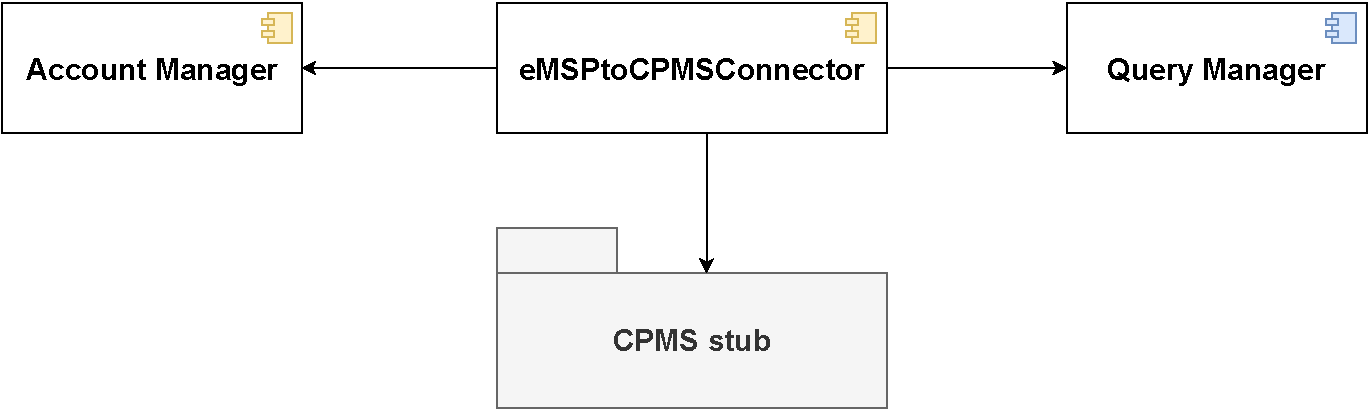
\includegraphics[scale=0.6]{src/Integration/eMSPConnector.pdf}
    \caption{Connector Subsystem}
\end{figure}
Then the following subsystems could be developed in any order or in parallel because they are decoupled. All the components require
the eMSPtoCPMSConnector to simulate and test efficiently the implementation. 
The develop can start from the most complex tasks such as the Charging Point Manager and the Reservation Manager. 
Then the Suggestion Manager and the Car manager can be implemented.
\begin{figure}[H]
    \centering
    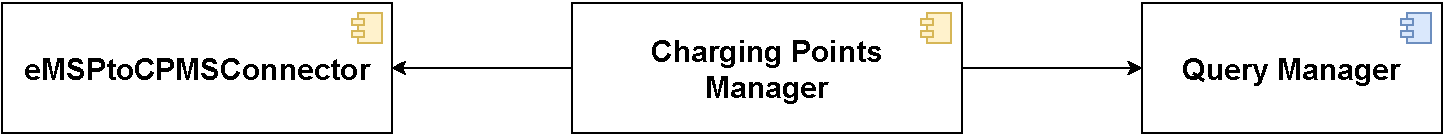
\includegraphics[scale=0.6]{src/Integration/eMSPCP.pdf}
    \caption{Charging Points Subsystem}
\end{figure}
\begin{figure}[H]
    \centering
    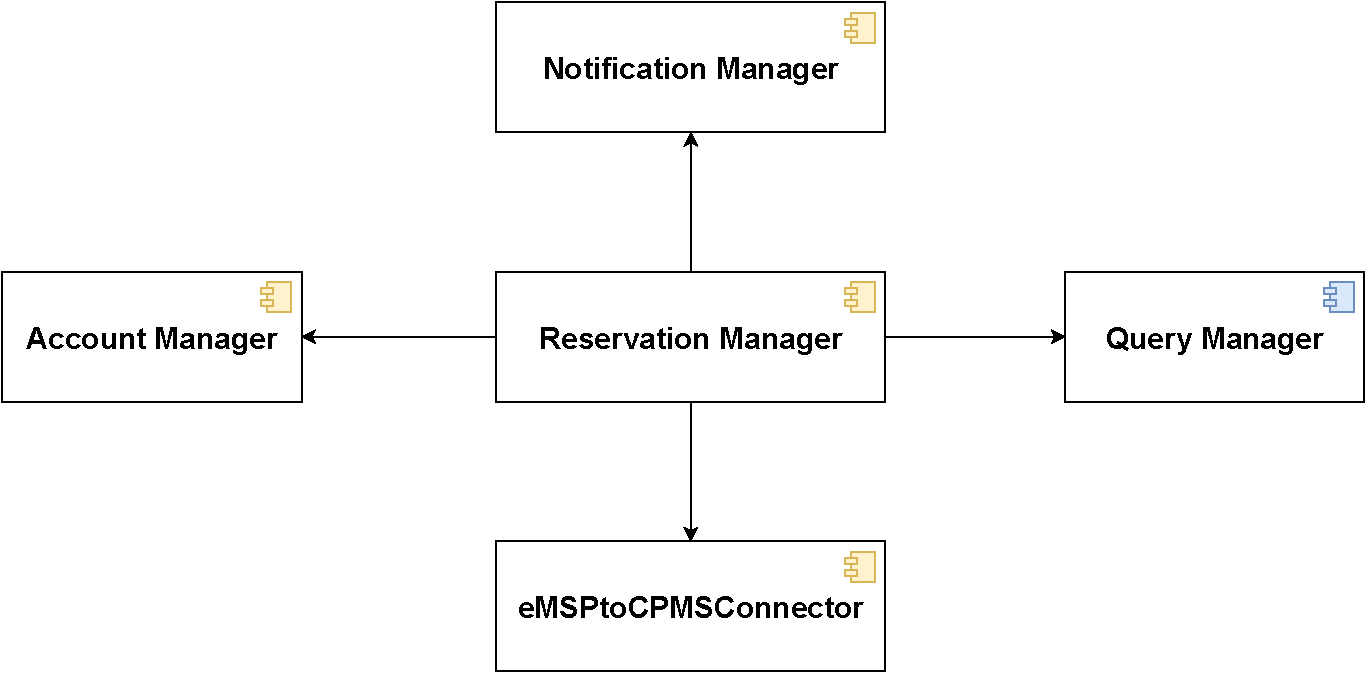
\includegraphics[scale=0.6]{src/Integration/eMSPReservation.pdf}
    \caption{Reservation Subsystem}
\end{figure}
\begin{figure}[H]
    \centering
    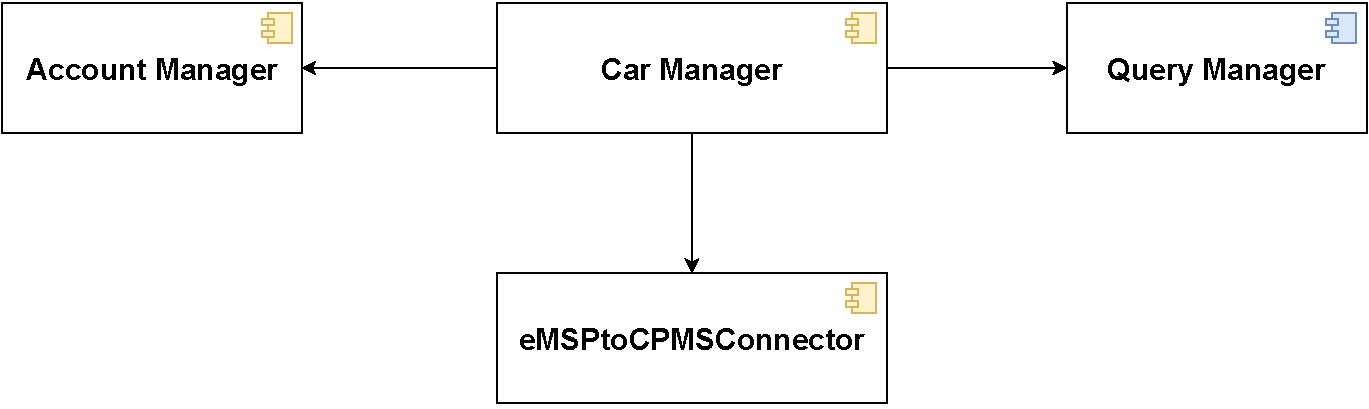
\includegraphics[scale=0.6]{src/Integration/eMSPCar.pdf}
    \caption{Car Subsystem}
\end{figure}
\begin{figure}[H]
    \centering
    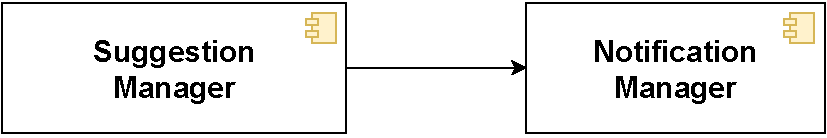
\includegraphics[scale=0.6]{src/Integration/eMSPSuggestion.pdf}
    \caption{Suggestion Subsystem}
\end{figure}
After having implemented and tested all the subsystems, the client and the eMSP can be integrated 
and tested together. 
\begin{figure}[H]
    \centering
    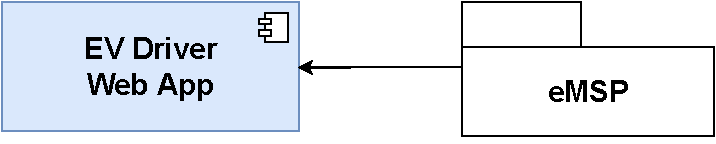
\includegraphics[scale=0.6]{src/Integration/eMSPFrontend.pdf}
    \caption{Client Application Integration}
\end{figure}


\subsubsection{CPMS}
The first components to be tested together are the Query Manager and the DBMS as they are the
components necessary for all the others when handling data.
\begin{figure}[H]
    \centering
    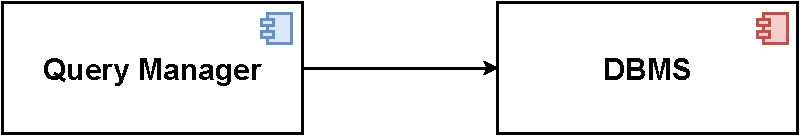
\includegraphics[scale=0.6]{src/Integration/CPMSQuery.pdf}
    \caption{Data Subsystem}
\end{figure}
Then it can be implemented the Account Manager that provides the account managing functions and the authorization interface 
to verify the permissions to do operations with the other components. It handles personal CPO's data and for this reason needs
to be tested carefully.
\begin{figure}[H]
    \centering
    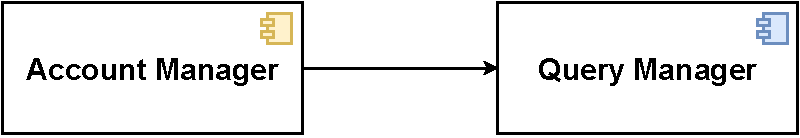
\includegraphics[scale=0.6]{src/Integration/CPMSAccount.pdf}
    \caption{Account Subsystem}
\end{figure}
The CPMStoeMSPConnector can be implemented after the Account Manager, a stub of the eMSP can be implemented at this point to simulate
the requests coming from the eMSP on the other side of the communication. This stab is an exception to the bottom-up approach, but
enables the possibility to develop separately the eMSP and the CPMS. 
\begin{figure}[H]
    \centering
    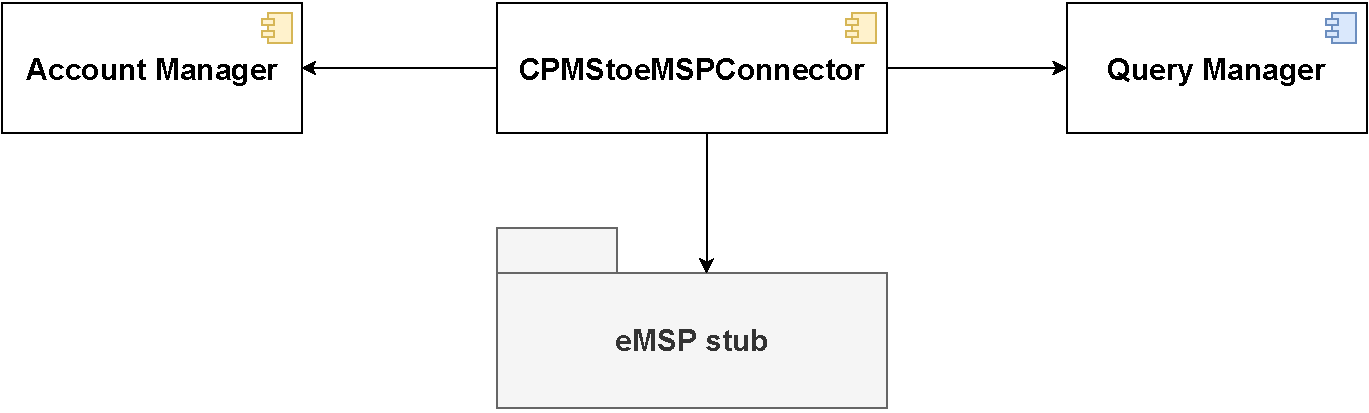
\includegraphics[scale=0.6]{src/Integration/CPMSConnector.pdf}
    \caption{Connector Subsystem}
\end{figure}
Then can be implemented the Rates Manager that offers an interface to create and modify rates that
are later associated with the CPs.
\begin{figure}[H]
    \centering
    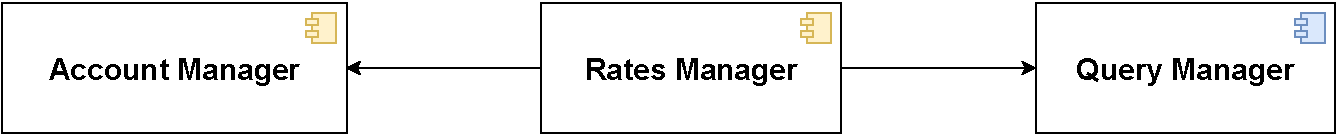
\includegraphics[scale=0.6]{src/Integration/CPMSRates.pdf}
    \caption{Rates Subsystem}
\end{figure}



\subsection{System Testing}
Eventually, when the integration of the components have taken place take place the testing of the entire System. 
The aim is to verify the functional and non-functional requirements and must take place in a testing
environment that is as close as possible to the production environment. 
The eMall System will undergo the following test:
\begin{itemize}
    \item \textbf{Functional testing}: The system is tested against the functional requirements and specification 
    specified on the RASD document.
    \item \textbf{Performance testing}: Check wether a software remains functional with increase demand and 
    various environment conditions.
\end{itemize}

\section{Effort Spent}
\subsection*{Pair working}
\begin{table}[H]
    \begin{tabular}{lr}
        \toprule
        \textbf{Project Specification Analysis, Brainstorming, RASD structure} & \textbf{4h} \\
        \textbf{Study of the context and existing protocols}                   & \textbf{5h} \\
        \textbf{Goals and Phenomena listing}                                   & \textbf{3h} \\
        \textbf{Use cases diagrams and description}                            & \textbf{7h} \\
        \textbf{Sequence diagrams}                                             & \textbf{8h} \\
        \textbf{Final Review}                                                  & \textbf{5h} \\
        \bottomrule
    \end{tabular}
\end{table}

\subsection*{Giovanni}
\begin{table}[H]
    \begin{tabular}{lr}
        \toprule
        \textbf{Definitions, Acronyms}          & \textbf{1.5h} \\
        \textbf{Assumptions, dependencies}      & \textbf{2.5h} \\
        \textbf{Mapping on goals, on use cases} & \textbf{3h}   \\
        \textbf{Non-functional requirements}    & \textbf{2.5h} \\
        \textbf{Formal Analysis with Alloy}     & \textbf{8h}   \\
        \bottomrule
    \end{tabular}
\end{table}

\subsection*{Matteo}
\begin{table}[H]
    \begin{tabular}{lr}
        \toprule
        \textbf{...} & 2.5h \\
        \textbf{...} & 4h   \\
        \textbf{...} & 2.5h \\
        \textbf{...} & 6h   \\
        \textbf{...} & 7.5h \\
        \bottomrule
    \end{tabular}
\end{table}

\subsection*{Lorenzo}
\begin{table}[H]
    \begin{tabular}{lr}
        \toprule
        \textbf{Scenarios}                     & \textbf{3h} \\
        \textbf{Class Diagram}                 & \textbf{1h}   \\
        \textbf{State Diagrams}                & \textbf{2.5h} \\
        \textbf{User Interfaces}               & \textbf{17h}   \\
        \textbf{Review}                        & \textbf{4h}   \\
        \bottomrule
    \end{tabular}
\end{table}

\section{References}
\begin{itemize}
    \item PWA
    \begin{itemize}
        \item \url{https://web.dev/progressive-web-apps/}
        \item \url{https://developer.mozilla.org/en-US/docs/Web/Progressive_web_apps}
    \end{itemize}
\end{itemize}

\end{document}